\documentclass[12pt, twoside]{article}
\setcounter{secnumdepth}{3}
\usepackage{jmlda}
\newcommand{\hdir}{.}

\renewcommand{\baselinestretch} {1.35}
\usepackage{xcolor}

\usepackage[english, russian]{babel}
\usepackage[utf8]{inputenc}

% The package for images
\usepackage{graphics}
\usepackage{graphicx}
\usepackage{caption}
\usepackage{subfig}
\graphicspath{{phase/}}
\DeclareGraphicsExtensions{.pdf,.png,.jpg}

% Доп пакеты
%\usepackage[usenames]{color}
\usepackage{colortbl}
\usepackage{enumitem}
\setlist{nolistsep}%, itemsep=0.1cm, parsep=0pt}
% The package for text in angle
\usepackage{booktabs}

% The package for Gothic letters
\usepackage{amssymb}

% The algorithmicx package for pseudocode
\usepackage{algorithm} 
\usepackage{algorithmic} 


\newcommand{\N}{\mathbb{N}}
\newcommand{\Z}{\mathbb{Z}}
%https://www.overleaf.com/project/6034bac8be0902011ffeee39
\theoremstyle{definition}

\newenvironment{theorem}[2][Теорема]{\begin{trivlist}
\item[\hskip \labelsep {\bfseries #1}\hskip \labelsep {\bfseries #2.}]}{\end{trivlist}}
\newenvironment{lemma}[2][Lemma]{\begin{trivlist}
\item[\hskip \labelsep {\bfseries #1}\hskip \labelsep {\bfseries #2.}]}{\end{trivlist}}
\newenvironment{exercise}[2][Задача]{\begin{trivlist}
\item[\hskip \labelsep {\bfseries #1}\hskip \labelsep {\bfseries #2.}]}{\end{trivlist}}
\newenvironment{reflection}[2][Reflection]{\begin{trivlist}
\item[\hskip \labelsep {\bfseries #1}\hskip \labelsep {\bfseries #2.}]}{\end{trivlist}}
\newenvironment{proposition}[2][Proposition]{\begin{trivlist}
\item[\hskip \labelsep {\bfseries #1}\hskip \labelsep {\bfseries #2.}]}{\end{trivlist}}
\newenvironment{corollary}[2][Corollary]{\begin{trivlist}
\item[\hskip \labelsep {\bfseries #1}\hskip \labelsep {\bfseries #2.}]}{\end{trivlist}}


\def\eps{\varepsilon}
\def\T{{\cal T}}
\def\H{{\cal H}}
\def\K{{\cal K}}
\def\L{{\cal L}}
\def\F{{\cal F}}
\def\Q{{\cal Q}}
\def\N{{\cal N}}
\def\p{{\cal P}}
\def\np{{\cal NP}}
\def\A{{\cal A}}
\def\B{{\cal B}}
\def\D{{\cal D}}
\def\BB{{\cal B}^* }
\def\DD{{\cal D}^* }
\def\TT{\tilde{\cal T}}
\def\f{\tilde f}
\def\ind{\mathop{\rm index}}
\def\St{\mathop{\rm St}}
\let\bd\partial
\def\V{\ensuremath{{\cal V}}}
\def\SS{{\mathbb S}}
\def\RR{\mathbb R}
\def\QQ{\mathbb Q}
\def\PP{\mathbb P}
\def\AA{\mathbb A}
\def\R{\cal R}
\def\NN{\mathbb N}
\def\CC{\mathbb C}
\def\ZZ{\mathbb Z}
\def\s{\sigma}
\def\S{\Sigma }
\def\ss{\Sigma^* }
\def\ra{\rightarrow}
\def\da{\downarrow}
\def\Ra{\Rightarrow}
\def\t{\theta}

\begin{document}

\title
    [] % краткое название; не нужно, если полное название влезает в~колонтитул
    {Восстановление фазы движения человека по сигналам носимых устройств}
\author
    [А.\,Д.~Курдюкова] % список авторов (не более трех) для колонтитула; не нужен, если основной список влезает в колонтитул
    {А.\,Д.~Курдюкова$^{1}$, Г.\,В.~Кормаков$^{2, 3}$, Д.\,М.~Тихонов$^{1}$, В.\,В.~Стрижов$^{1, 4}$} % основной список авторов, выводимый в оглавление
    % [А.\,Д.~Курдюкова, Г.\,В.~Кормаков, Д.\,М.~Тихонов, В.\,В.~Стрижов] % список авторов, выводимый в заголовок; не нужен, если он не отличается от основного
\email
   {kurdiukova.ad@phystech.edu; kormakov\_georgiy@forecsys.ru; tihonov.dm@phystech.edu;  strijov@ccas.ru}
% \thanks
%     {Работа выполнена при 
%     %частичной
%     финансовой поддержке РФФИ, проекты \No\ \No 00-00-00000 и 00-00-00001.}
\organization
{$^1$Московский физико-технический институт
(национальный исследовательский университет)\\
$^2$Московский государственный университет имени М.В.Ломоносова\\ 
$^3$ООО <<Форексис>>, Москва, ул.Вавилова, 42;\\
$^4$Вычислительный Центр им. А.А. Дородницына РАН }
\abstract
  {\textbf{Аннотация}:
  Решается задача восстановления фазы квазипериодических сигналов движения человека. Эти сигналы имеют повторяющиеся значения без явной периодичности. Предлагается алгоритм определения фазы движения. Он основан на представлении исходного временного ряда в фазовом пространстве. Строится траекторная матрица временного ряда. Предлагается критерий выбора оптимальной размерности траекторного пространства. Значения фазы присваиваются в соответствии с близостью точек временного ряда к аппроксимирующей модели. Результаты работы алгоритма демонстрируется на сигналах, полученных с трехосевого акселерометра. Используются пять классов периодического движения человека. Для анализа качества работы алгоритм сравнивается с методом, использующим максимумы автокорелляционной функции.

%Вводится понятие возмущения фазы. Исследуется работа алгоритма при данном явлении.

\bigskip
\noindent
\textbf{Ключевые слова}: \emph {анализ поведения, восстановление фазы, временные ряды, фазовая траектория, траекторное пространство, метод главных компонент}
}

%данные поля заполняются редакцией журнала
\doi{}
\receivedRus{}
\receivedEng{}

\maketitle
\linenumbers
%%%%%%%%%%%%%%%%%%%%%%%%%%%%%%%%%%%%%%%%%%%%%%%%%%%%%%%%%%%%%%%%%%%%%%%%%%%%%%%%
\section{Введение}
Решается задача анализа квазипериодических сигналов, считываемых с носимых устройств.
Временной ряд $\{s_i\}_{i=1}^N$\, назовем \emph{квазипериодическим} с периодом $T$, если для каждого $i$, такого что $i + T \geq N$, найдется ошибка $\varepsilon$, такая что выполнено
\begin{equation}\label{st}
  \{s_i\}_{i=1}^N, \quad s_{i} = s_{[i + T]} + \varepsilon.
\end{equation}

Исследование фазы является важной частью анализа временных рядов. Целью данной работы является построение алгоритма извлечения фазы квазипериодического временного ряда. Зная фазу периодического или квазипериодического временного ряда, можно сегментировать временной ряд по периоду. Задача восстановления фазы сигнала встречается в прикладной физике, кристаллографии~\cite{kim1991phase, hauptman1991phase, millane1990phase}, астрономии~\cite{fienup1987phase, bruck1979ambiguity}, лазерной оптике~\cite{seifert2004nontrivial, seifert2006multilevel}. 

В вычислительном эксперименте исследуются ходьба, бег трусцой и другие типы походки человека \cite{jansi2018novel, khan2010triaxial, ignatov2016human}. Результаты анализа этих данных используются для распознавания человеческой активности \cite{bevilacqua2018human, jansi2018novel, lu2017towards, ordonez2016deep, sun2018sequential, wang2020wearable}, в медицинских приложениях \cite{bussmann1998ambulatory, najafi2003ambulatory}, при мониторинге состояния пациентов \cite{grunerbl2014smartphone}, для обнаружения падений пожилых людей \cite{ma2014depth}.

Для извлечения фазы временных рядов периодических процессов требуется ручная маркировка. Однако этот метод неприменим для временных рядов больших размеров. Существуют более универсальные способы определения фазы. Например, в~\cite{jatesiktat2017unsupervised} применяется двойной автоэнкодер.

В~\cite{yang1994gerchberg, guo2015iterative, seifert2006multilevel, jatesiktat2018unsupervised} представлены альтернативные алгоритмы определения фазы. Итеративный алгоритм Герхберга-Сакстона~\cite{yang1994gerchberg} с использованием прямого и обратного преобразований Фурье. Его модификации описаны в~\cite{guo2015iterative}. Они заключаются в улучшении сходимости базового алгоритма, а также в добавлении случайного возмущения фазы на каждой итерации для избежания сходимости к неверному решению. Многоуровневые методы Гаусса-Ньютона~\cite{seifert2006multilevel} основаны на линейной В-сплайн аппроксимации с итеративным применением локального метода Гаусса-Ньютона. Метод извлечения фаз, основанный на неконтролируемом обучении, представлен в~\cite{jatesiktat2018unsupervised}.

В работах \cite{motrenko2015extracting, ignatov2016human, grabovoy2020quasi} решается задача сегментации квазипериодических временных рядов. Строится низкоразмерное фазовое пространство.
В \cite{motrenko2015extracting, grabovoy2020quasi} размерность этого подпространства фиксирована и равна двум.
Выбор размерности опирается на теорему, доказанную в~\cite{motrenko2015extracting}. Теорема посвящена утверждению об аппроксимации периодических компонент синусоидального временного ряда. %с периодом ~$T > 2 [timestamps]$.
В реальных данных встречается суперпозиция нескольких главных компонент. Для подобных сигналов теорема неприменима.
Размерность собственного подпространства, равная двум, не является достаточной для построения устойчивой модели.
В работе \cite{ignatov2016human} осуществляется переход к признаковому описанию точек исходного временного ряда. В фазовом пространстве используются метрики.
В случае пространства высокой размерности данный подход неустойчив из-за проклятия размерности \cite{bellman1957dynamic, bellman1961adaptive, beyer1999nearest, powell2007approximate}. 

В данной работе для нахождения фазы осуществляется переход в фазовое пространство с помощью метода задержек \cite{lukyanov, maltsev}. В качестве примера на Рис.~\ref{fg:initial_traj} изображен синтетический временной ряд $s(t) = \sin t$. Его фазовая траектория изображена в трехмерном пространстве. 

\begin{figure}[ht]
\centering
  \subfloat[Временной ряд]{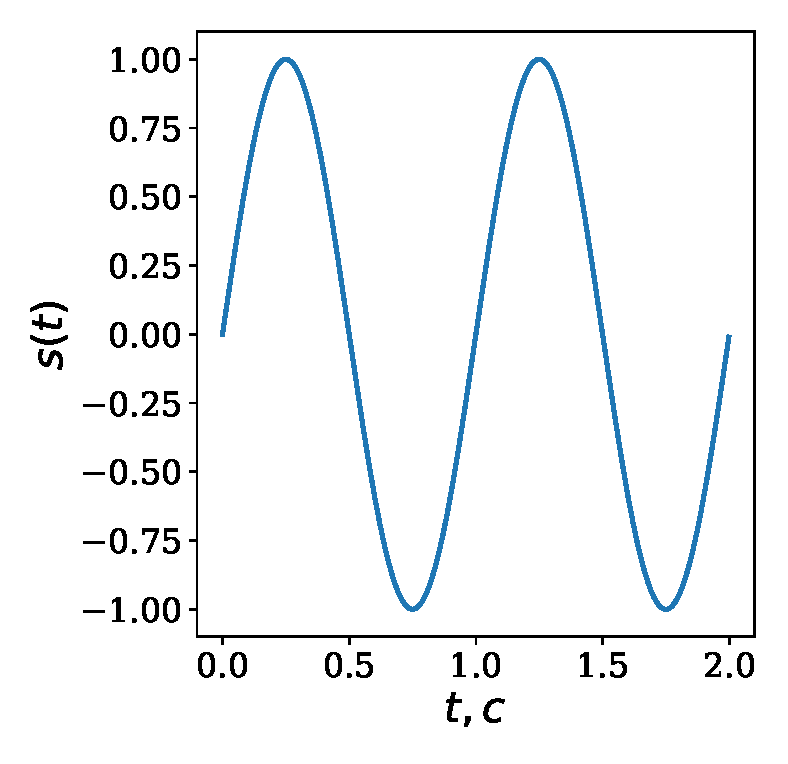
\includegraphics[width=0.3\textwidth]{./images/synthetic_example.eps}}
  \subfloat[Фазовая траектория (PCA)]{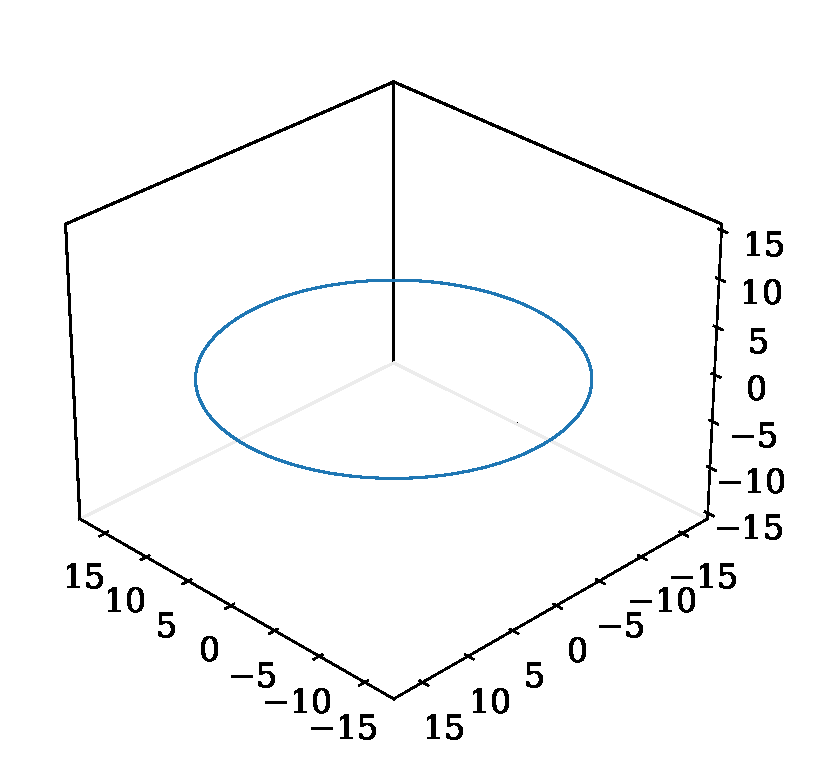
\includegraphics[width=0.3\textwidth]{./images/synthetic_trajectory.eps}}\\
\caption{Синусоидальный временной ряд и его фазовая траектория в 3D. }
\label{fg:initial_traj}
\end{figure}
 
В \cite{motrenko2015extracting, grabovoy2020quasi, usmanova} показана избыточность исходного фазового пространства. Под \emph{избыточностью фазового подпространства} понимается следующее. При переходе в фазовое подпространство ошибка восстановленных значений мала по сравнению с амплитудой исходного временного ряда.

Фиксированное значение фазовой траектории интерпретируется как начальная фаза класса движения, если это значение повторяется в фазовом пространстве с точностью до допустимой ошибки. 
Предполагается, что в собственном подпространстве возможно более \emph{устойчивое извлечение начальной фазы.}
При увеличении амплитуды случайных отклонений исходного временного ряда модель, определяющая фазу, не изменяет существенно своего прогноза.   

\begin{table}
% \label{table:comparison}
\begin{tabular}{|p{7.5cm}|p{7.5cm}|}
\hline
Преимущества & Недостатки\\
\hline
\multicolumn{2}{|c|}{\textit{Максимумы автокорреляционной функции}}\\
\hline
    Простота, & Неустойчивость к частотным и амплитудным шумам,\\
    интерпретируемость. & затухание на длительный рядах.\\
    
\hline
\multicolumn{2}{|c|}{\textit{Герхберга-Сакстона \cite{gerchberg1972practical}}}\\
\hline
    ??Устойчивость к частотным и фазовым шумам??, & Ограниченность базиса из $\sin$ и $\cos$,\\
    сходимость. & зависимость от доп. информации об ограничениях на образ преобразования Фурье,\\
     & ресурсоемкость.\\
  
\hline
\multicolumn{2}{|c|}{\textit{Дуальный автоэнкодер \cite{jatesiktat2020unsupervised}}}\\
\hline
    Устойчивость к частотным и амплитудным шумам, & Неинтерпретируемость,\\
    не требует доп. информации о сигнале. & ресурсоемкость.\\
\hline
\multicolumn{2}{|c|}{\textit{Преобразование Гильберта \cite{kak1973hilbert}}}\\
\hline
     Простота,&Неустойчивость к частотным и амплитудным шумам,\\
     интерпретируемость, & ограниченность только синусоидальными сигналами.\\
     отсутствие необходимости в доп. информации о сигнале.&\\
\hline
\multicolumn{2}{|c|}{\textit{Предлагаемый в данной работе подход}}\\
\hline
Интерпретируемость, & Вычислительно затратный алгоритм,\\
устойчивость по отношению к изменению амплитуды и частоты,  & необходимость в дополнительной информации о сигнале (знание первого периода).\\
устойчивость.& \\
\hline
\end{tabular}
\caption{\label{tab:table-name}Сравнительный анализ алгоритмов восстановления фазы.}
\end{table}


В таблице 1 приведен список методов, решающих задачу восстановчления фазы. Перечислены их преимущества и недостатки, упомянут предлагаемый в данной работе.

Предлагаемый алгоритм прогнозирует фазу временного ряда периодического движения человека. Класс периодического движения фиксирован. Алгоритм работает в пространстве оптимальной размерности.
В работе описан критерий оптимальной размерности, который опирается на условие отсутствия \emph{самопересечений} в фазовом пространстве. Будем говорить, что в фазовом подпространстве отсутствуют самопересечения, если ожидаемое значение траектории не имеет пересечений в пределах среднеквадратичного отклонения.

%%%%%%%%%%%%%%%%%%%%%%%%%%%%%%%%%%%%%%%%%%%%%%%%%%%%%%%%%%%%%%%%%%%%%%%%%%%%%%%%
\section{Постановка задачи}
Алгоритм извлечения фазы, предлагаемый в данной работе, использует представление временного ряда в фазовом пространстве. Такое представление описано, например, в~\cite{usmanova}. В этой же статье вводится понятие избыточности фазового пространства, что приводит к неустойчивой работе алгоритма. Поэтому целью является переход в пространство фаз сниженной размерности. 

% Данные, считанные с трехосевого акселерометра, представляют собой временной ряд 
% \begin{equation}
% \label{ts_3}    
%     \{ \mathbf{a}_i \}_{i = 1}^{N},
%     \quad \mathbf{a}_i =
%     \begin{bmatrix}
%     a_{ix} \; a_{iy} \;a_{iz}
%     \end{bmatrix}^{T},
%     \quad \mathbf{a}_i \in \RR^3.
% \end{equation}
% Частота сэмплирования $\nu$ фиксирована.\\
В работе рассматривается временной ряд~\eqref{st}. Значение ряда в момент времени $i$
    \begin{equation}\label{ts}
        s_i = \sqrt{a_{ix}^2 + a_{iy}^2 + a_{iz}^2},
    \end{equation}
В формуле \eqref{ts} $\nu$ -- частота сэмплирования, $a_{ix},\,a_{iy},\,a_{iz}$ -- данные, считанные с трехосевого акселерометра.
Предполагается, что он соответствует фиксированному классу периодического движения~ $y\in\mathbb{Y}\,$. Таковыми являются, например, ходьба, приседания, подъем или спуск по лестнице, велопрогулка. То есть предполагается отсутствие момента изменения характеристик сигнала, который относил бы его к другому классу.
Для анализа периодических компонент ряда~\eqref{st} и перехода в собственное пространство строится его траекторная матрица $\mathbf{H}$.

    \[ \mathbf{H} = \begin{bmatrix}
                        s_1 & \dots & s_n \\
                        s_2 & \dots & s_{n+1} \\
                        \vdots  &\ddots& \vdots \\
                        s_{k} & \dots & s_{N}
                    \end{bmatrix}^{\mathffs{T}} = 
                    \begin{bmatrix}
                        \mathbf{s}_1,
                        \mathbf{s}_2, 
                        \dots,
                        \mathbf{s}_k
                    \end{bmatrix}, \quad k = N - n + 1, \]
где~$n$ -- ширина окна, не меньшая, чем предполагаемый период: $n\nu \geq T$.

Размерность исходного фазового пространства избыточна.
Осуществляется переход в собственное подпространство меньшей размерности.
    \[ \mathbf{X} = \mathbf{W}^{\mathfs{T}} \mathbf{H} = \begin{bmatrix}
                        \mathbf{x}_1,
                        \mathbf{x}_2,
                        \dots,
                        \mathbf{x}_k 
                    \end{bmatrix}, \quad \mathbf{x}_i\in \RR^p, \,  \]
где $\mathbf{W}$ --- матрица преобразования алгоритма PCA. Число выбранных компонент равно $p$. Они соответствуют наибольшим собственным значениям.

Требуется построить модель $m: \varphi \rightarrow \mathbf{x}$, аппроксимирующую фазовую траекторию с помощью минимального числа главных компонент.
С помощью аппроксимирующей модели определить критерий выбора оптимальной размерности фазового подпространства. На основе критерия и модели предложить алгоритм нахождения устойчивой фазы.
%%%%%%%%%%%%%%%%%%%%%%%%%%%%%%%%%%%%%%%%%%%%%%%%%%%%%%%%%%%%%%%%%%%%%%%%%%%%%%%%
\section{Определение фазы в пространстве оптимальной размерности}
В данном разделе вводится понятие оптимальной размерности фазового подпространства и дается описание алгоритма определения фазы.
В параграфе \textbf{3.1} определена модель средней траектории ряда и ее дисперсии, которые нужны для определения критерия выбора размерности траекторного пространства в параграфе \textbf{3.2} и функций потерь в параграфе \textbf{3.3}.
Описанию алгоритма определения фазы посвящен параграф \textbf{3.4}.

\paragraph{Модель фазовой траектории} \label{subsection:4.1}
Аппроксимирующая модель математического ожидания фазовой траектории $\Expect(\mathbf{x}|\varphi):~\varphi~\rightarrow~\mathbf{x}$ ставит в соответствие фазе $\varphi \in [0, 2\pi]$ точку в фазовом подпространстве $ \mathbf{x}\in\RR^p$. 
В качестве аппроксимирующей модели предлагается регрессия Надарая-Ватсона

\begin{equation}           
    m(\varphi) = \Expect(\mathbf{x}|\varphi) =
        \frac{\sum_{\mathbf{x'}\in \mathbf{X}}  \mathbf{x'} \cdot K\left(\frac{\rho(\varphi^{\mathbf{x'}}_{\text{estimated}}, \varphi)}{h}\right)}
        {\sum_{\mathbf{x'}\in \mathbf{X}} K\left(\frac{\rho(\varphi^{\mathbf{x'}}_{\text{estimated}}, \varphi)}{h}\right)},
\label{eq:NW} 
\end{equation}

\begin{equation}           
    m(\varphi) = \Expect(\mathbf{x}|\varphi) =
        \frac{\int_{\mathbf{x'}\in \mathbf{X}}  \mathbf{x'} \cdot K\left(\frac{\rho(\varphi^{\mathbf{x'}}_{\text{estimated}}, \varphi)}{h}\right) d\mathbf{x'}}
        {\int_{\mathbf{x'}\in \mathbf{X}} K\left(\frac{\rho(\varphi^{\mathbf{x'}}_{\text{estimated}}, \varphi)}{h}\right) d\mathbf{x'}},
\label{eq:NW2} 
\end{equation}
где $h$ -- фиксированная ширина окна, $\rho$~-- метрика в пространстве фаз и $K$ -- ядро.
В формуле \eqref{eq:NW} $\varphi^{\mathbf{x'}}_{\text{estimated}}$ -- начальное приближение фазы для каждой точки $\mathbf{x'}$ первого периода.
% , которое строится на основе знания о примерном значении одного периода. По автокорреляционной функции можно определить индекс $i_{\text{init}}$ для пика и индекс $i_{\text{final}}$ для пика конца первого периода. Тогда начальное приближение $\varphi^{\mathbf{x'}}_{\text{estimated}}$ строится линейным приближением между индексами $i_{\text{init}}$ и $i_{\text{final}}$.

Аналогично предлагается ввести и модель дисперсии $\Variance$:

\begin{equation}           
    d(\varphi) = \Variance(\mathbf{x}|\varphi) =
        \frac{
        \sum_{\mathbf{x'}\in \mathbf{X}}  \|\mathbf{x'} - \Expect(\mathbf{x}|\varphi)\|_2
        \cdot
        K\left(\frac{\rho(\varphi^{\mathbf{x'}}_{\text{estimated}}, \varphi)}{h}\right)
        }
        {\sum_{\mathbf{x'}\in \mathbf{X}} K\left(\frac{\rho(\varphi^{\mathbf{x'}}_{\text{estimated}}, \varphi)}{h}\right)
        },
\label{eq:NW3} 
\end{equation}

\begin{equation}           
    d(\varphi) = \Variance(\mathbf{x}|\varphi) =
        \frac{
        \int_{\mathbf{x'}\in \mathbf{X}}  
        \|\mathbf{x'} - \Expect(\mathbf{x}|\varphi)\|_2
        \cdot
        K\left(\frac{\rho(\varphi^{\mathbf{x'}}_{\text{estimated}}, \varphi)}{h}\right) 
        d\mathbf{x'}
        }
        {\int_{\mathbf{x'}\in \mathbf{X}} K\left(\frac{\rho(\varphi^{\mathbf{x'}}_{\text{estimated}}, \varphi)}{h}\right) d\mathbf{x'}},
\label{eq:NW4} 
\end{equation}
В качестве ядра используется радиальная базисная функция:

\[ K(r)= \exp\left(-\gamma\| r \|^2\right). \]
В качестве полуметрики в пространстве фаз:

    \[ \rho(\varphi_1, \varphi_2) = \frac{1 - \cos(\varphi_1 - \varphi_2)}{2},
    \quad
    \varphi_1,\,\varphi_2 \in [0, 2\pi).\]

Модели для $\Variance(\mathbf{x}|\varphi)$ и $\Expect(\mathbf{x}|\varphi)$ необходимы для введения критерия выбора оптимальной размерности подпространства и функций потерь в последующих разделах.

\paragraph{Критерий выбора оптимальной размерности фазового подпространства} \label{subsection:4.2}
Поиск минимальной необходимой размерности траекторного подпространства позволяет построить адекватную аппроксимацию ряда~\eqref{ts}. В найденном пространстве оптимальной размерности строится алгоритм восстановления фазы временного ряда.

\textbf{Определение.}
Значения фазы называются \textit{существенно разными}, если их разность превосходит $\frac{\pi}{3}$.
Фазовая траектория имеет точки \textit{самопересечение}, если они имеют  существенно разную фазу и расположены на расстоянии, меньшем суммы дисперсий в этих точках.

Для определения критерия оптимальной размерности введем множество фаз $\Phi(p)$, таких что норма разности между соответствующей и текущей точками модельной траектории $\|\Expect(\mathbf{x}|\varphi) - \Expect(\mathbf{x}|\varphi')\|_2$ не превосходит суммы дисперсий этих точек $\Variance(\mathbf{x}|\varphi) + \Variance(\mathbf{x}|\varphi')$, а значения фаз $\varphi$ и $\varphi'$ отличаются более, чем на $\frac{\pi}{2}$, но менее, чем на $\frac{3\pi}{2}$:

\begin{align}           
    \Phi(p) = \{\varphi |
    \quad
    \|\Expect(\mathbf{x}|\varphi) - \Expect(\mathbf{x}|\varphi')\|_2
    \leq
    \Variance(\mathbf{x}|\varphi) + \Variance(\mathbf{x}|\varphi'),
    \nonumber \\
    \frac{\pi}{2} \leq |\varphi - \varphi'| \leq \frac{3\pi}{2},
    \quad
    \varphi,\varphi' \in [0,2\pi),
    \quad
    \mathbf{x} \in \mathbb{R}^p
    \}
\label{eq:intersection} 
\end{align}

% \begin{align} 
%     I(p) = \{\varphi|
%     \quad
%     \|\Expect(\mathbf{x}|\varphi) - \Expect(\mathbf{x}|\varphi')\|_2
%     \leq
%     \Variance(\mathbf{x}|\varphi) + \Variance(\mathbf{x}|\varphi'),
%     \\
%     \rho (\varphi,\varphi') \leq \frac{1}{2},
%     \quad
%     \varphi,\varphi' \in [0,2\pi),
%     \quad
%     \mathbf{x} \in \mathbb{R}^p
%     \}
% \label{eq:intersection2} 
% \end{align}

\textbf{Определение.}
Оптимальная размерность пространства - это размерность пространства, в которой выполняется критерий отсутствия самопересечений.

\textbf{Определение.}
Критерием оптимальной размерности в пространстве называется

\begin{equation}           
    \hat{p} = \arg\min_{p \in \{1, \dots, n \}} |\Phi(p)|,
\label{eq:intersection_criterion} 
\end{equation}
где $n$ - размерность исходного пространства.\\


\paragraph{Функция потерь для определения фазы} \label{subsection:4.3}

Основная идея алгоритма заключается в присвоении фазы новым точкам временного ряда в соответствии с их близостью с аппроксимирующей моделью в фазовом пространстве.  

Предположения:
\begin{enumerate}
    \item Во временном ряде~\eqref{st} присутствует только один фиксированный класс движений; 
    
    \item \label{enum:2} Более поздним по времени точкам в пределах одного периода соответствует б\'{о}льшая фаза.  
    Если $t > t'$, то $\varphi_t > \varphi_{t'}$ для~$t,\, t' \in [0,+\infty)$;
    
    \item \label{enum:3} Фазы соседних точек близки. Если $\| \mathbf{x} - \mathbf{x}' \|_2 < \eps$ ($\eps$ -- гиперпараметр), то $| \varphi - \varphi'|<\delta$ для некоторого $\delta$.
\end{enumerate}

Предлагается определять значение фазы, исходя из следующих функций потерь.

Функция потерь $L_1$ опирается на предположение~\ref{enum:2} о монотонном росте фаз:

\begin{equation}      
    L_1(\varphi) =
    \begin{cases}
        \frac{1-\cos(\varphi-\varphi')}{2},\;
            \text{если } \varphi \geq \varphi' \;\text{при}\; t' \geq t\\
        0, \;
            \text{иначе.}
    \end{cases},
\label{eq:L1} 
\end{equation}

% Возможен вариант назначения штрафа в масштабах расстояния между точками $\mathbf{x}'$ и $\mathbf{x}$ в фазовом пространстве

% \begin{equation}           
%     L_1(\varphi) = \begin{cases}
%                     \frac{\| \mathbf{x}' - \mathbf{x} \|}{D}, \; \text{если } \varphi \geq \varphi' \;\text{при}\; t' \geq t\\
%                     0, \; \text{иначе}
%     \end{cases}
% \label{eq:L1_1} 
% \end{equation}

Так как сигнал является квазипериодическим, то логично разрешить уменьшение фазы в пределах некоторой фиксированной величины $\delta_{\varphi}$. Тогда слагаемое $L_1(\varphi)$ можно записать в виде

\begin{equation}      
    L_1(\varphi) =
    \begin{cases}
        \frac{1-\cos(\varphi-\varphi')}{2},\;
            \text{если } \varphi - \varphi' \geq \delta_{\varphi} \;\text{при}\; t' \geq t\\
        0, \;
            \text{иначе.}
    \end{cases},
\label{eq:L1_2} 
\end{equation}


Функция потерь $L_2$ опирается на предположение~\ref{enum:3} о близости фазы соседних точек.

\begin{equation}           
    L_2(\varphi) = 
    \sum_{\| \mathbf{x} - \mathbf{x'} \|<\eps, \; \mathbf{x'} \in \mathbf{X}}
    \rho( \varphi, \varphi').
\label{eq:L2} 
\end{equation}
где $\eps$ - гиперпараметр, характеризующий максимальное расстояние между соседями в фазовом пространстве. 

    % Также можно учитывать некоторое фиксированное число $q$ точек $\mathbf{x}_j \in \mathbf{X}_{\text{history}}$ из предыстории ():
    
    % \begin{equation}           
    %     L_2(\varphi) = 
    %     \sum_{j\in\overline{1, q}}
    %     \rho( \varphi, f_{\text{history}}(\mathbf{x}_j)).
    % \label{eq:L2_1} 
    % \end{equation}
% Как вариант - ввести экспоненциальное забывание, где $\eta$ темп забывания
% \begin{equation}           
%     L_2^{(i)}(\varphi) = \eta\cdot\rho( \varphi_i, \varphi_{i-1}) + (1 - \eta)\cdot L_2^{(i-1)}.
% \label{eq:L2_2} 
% \end{equation}
Функция потерь $L_3$ учитывает расстояние от текущей точки до точек аппроксимирующей модели.
\begin{equation}           
    L_3(\varphi) = \frac{\|\mathbf{x} - m(\varphi)\|_2}{d(\varphi)}.
\label{eq:L3} 
\end{equation}

% Можно пробовать разные нормы, например
% \begin{equation}           
%     L_3(\varphi) = \frac{\|\mathbf{x}_i - f_{\text{approx}}(\varphi)\|_1}{D}, \quad L_3(\varphi) = \frac{\|\mathbf{x}_i - f_{\text{approx}}(\varphi)\|_{\infty}}{D}
% \label{eq:L3_1} 
% \end{equation}

Таким образом, задача нахождения фазы для текущей точки $\mathbf{x}_i$ имеет вид
\begin{equation} 
\widehat{\varphi}_i = \arg\min_{\varphi \in \Phi_i} \lambda_1\cdot L_1(\varphi) + \lambda_2 \cdot L_2(\varphi) + \lambda_3 \cdot L_3(\varphi).
\label{eq:argminL} 
\end{equation}
где $\lambda_1, \lambda_2, \lambda_3$ - весовые коэффициенты такие, что $\sum_{i=1}^{3} \lambda_i = 1$.

\paragraph{Алгоритм определения фазы} \label{paragraph:4.4}
% Предполагается, что помимо дискретного временного ряда известны индексы начала $i_{\text{start}}$ и конца $i_{\text{stop}}$ одного периода.
% Тогда точку временного ряда $\mathbf{x}_i$ и ее фазу $\varphi_{\text{apriori \;i}}$ поставим во взаимно однозначное соответствие по правилу:
% \begin{equation}
%     \varphi_{\text{apriori \;i}}  = 2\pi \cdot \frac{(i - i_{\text{start}})}{i_{\text{stop}} - i_{\text{start}}},
%     \quad
%     i\in \overline{i_{\text{start}}, i_{\text{stop}}}
% \label{eq:apr_phase}
% \end{equation}

Определим множество возможных фаз.
Для этого выберем такое множество точек в модели $f_{\text{approx}}$, в область отклонений которых попала текущая точка $\mathbf{x}_i$.
C помощью аппроксимирующей модели (\ref{eq:NW}) определим множество возможных фаз:

\begin{equation}           
    \mathbf{\Phi}_i = \left\{ \varphi\,:\|\mathbf{x}_i - f_{\text{approx}}(\varphi)\|_2\leq D,
    \quad
    \varphi \in [0,2\pi]\right\}
\label{eq:Phi_i} 
    \end{equation}

Введем конечное дискретное упорядоченное (по индексу вхождения) множество точек $\mathbf{X}_{\text{history}} \subset \mathbf{X}$, для которых фаза уже определена алгоритмом.
Аналогичное множество найденных фаз обозначим $\mathbf{\Phi}_{\text{history}}$.
Введем функцию $f_{\text{history}}: \mathbf{X}_{\text{history}} \rightarrow \mathbf{\Phi}_{\text{history}}$.

В данных обозначениях алгоритм определения фазы выглядит следующим образом (алгоритм \ref{algo:phase}).

%\begin{otherlanguage}{english}
\begin{algorithm}[!ht]
	\caption{Delay Embedding Phase Identifier}
	\begin{algorithmic}[1]
	\REQUIRE $s, \text{nlags}, \text{mindim}, \lambda_1,\lambda_2, \lambda_3$
    \ENSURE $\mathbf{\Phi}_{\text{history}}$
    \STATE На временном ряде $s$ построить автокорреляционную функцию с учетом ширины окна nlags для получения начального приближения
	\STATE По наибольшему пику определить начальное приближение мат. ожидания
	\STATE По первому периоду $f_{\text{approx}}$ согласно (\ref{eq:NW})
	\STATE По критерию найти пространство меньшей размерности и произвести в него переход по PCA с размерностью окна nlags
	\STATE Найти $\mathbf{\Phi}_{\text{history}}[1] = \min_{\phi \in [0,2\pi)}\|X[1] - m(\varphi)\|_2 $
	\WHILE{$|\mathbf{\Phi}_{\text{history}}| \neq |\mathbf{X}|$:}
	\STATE Найти множество возможных фаз согласно (\ref{eq:Phi_i})
	\STATE Найти ближайших соседей из предыстории (\ref{eq:L2})
	\STATE Найти минимум функции согласно  (\ref{eq:argminL})
	\STATE Добавить полученное значение в историю $\mathbf{\Phi}_{\text{history}}$
	\STATE Если был пройден 1 период, модель средней траектории обновляется по $\mathbf{\Phi}_{\text{history}}$.
	\ENDWHILE
	\end{algorithmic}
	\label{algo:phase}
\end{algorithm} 
%\end{otherlanguage}{english}
%%%%%%%%%%%%%%%%%%%%%%%%%%%%%%%%%%%%%%%%%%%%%%%%%%%%%%%%%%%%%%%%%%%%%%%%%%%%%%%%

\newpage

\section{Эксперимент}
Целью эксперимента является демонстрация результатов работы алгоритма.
Эксперименты проводились на реальных данных, полученных с акселерометра мобильного устройства. В качестве классов движения выбраны ходьба, приседания, движение вверх по лестнице и прогулке на велосипеде. Так же в эксперименте реализован критерий выбора оптимальной размерности.

В качестве проверки выбора оптимальной размерности фазового пространства построены графики зависимости функций ошибок от размерности фазового подпространства. Были выбраны функции ошибок MAPE и $R^2$ между истинными траекториями и восстановленными по компонентам оптимального фазового пространства. Графики представлены в таблице \ref{tbl:table_of_opt_dimension}. В большинстве случаев видно, что выбранная размерность не является избыточной. Это  подтверждается отсутствием самопересечений. При этом ошибка минимальна среди меньших размерностей. 

%По этим графикам согласно критерию $\mathfrak{K}$ определяется оптимальная размерность фазового подпространства для каждого класса движения. 
\begin{table}
    \centering
        \begin{tabular}{p{2.15cm}p{12cm}}
            \toprule
            Зависимость & ошибки $MAPE$ от размерности фазового подпространства\\
            \midrule
            \rotatebox{90}{ \text{Ходьба} }
            & 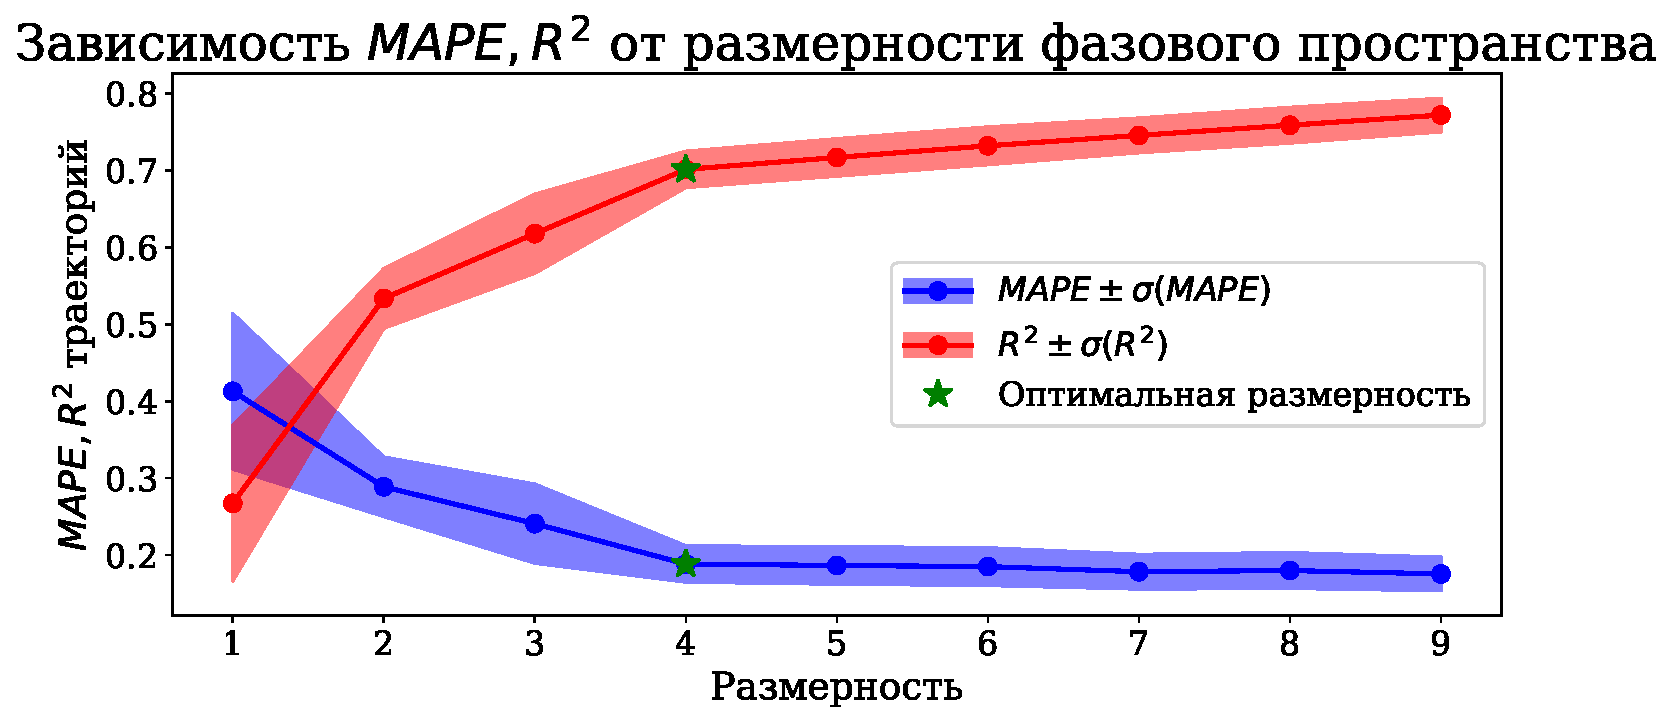
\includegraphics[scale=0.35]{./images/ru_mape_r2_p_walk.pdf}\\ 
            \hline
            
            \rotatebox{90}{ \text{Лестница} }
             & 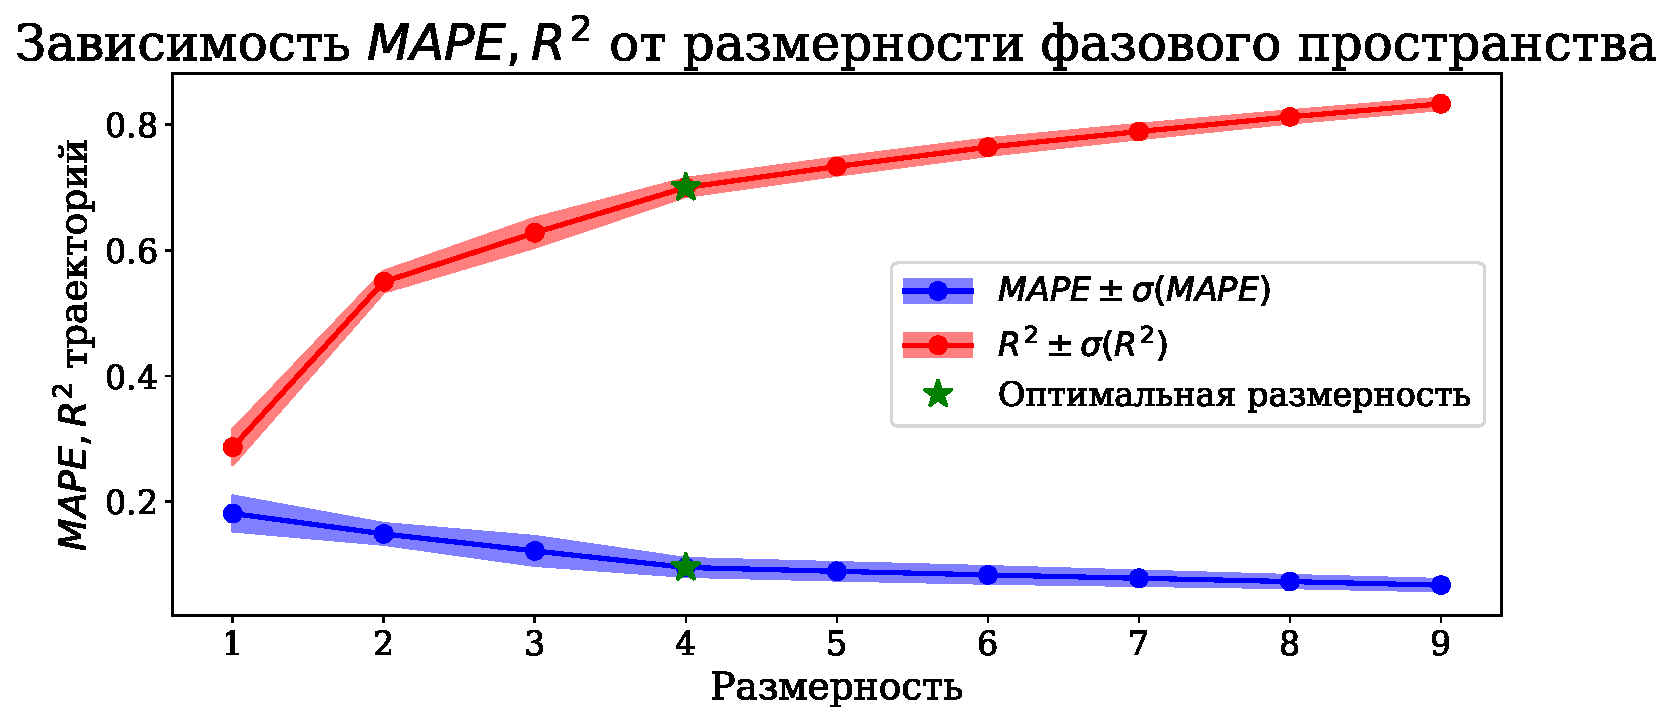
\includegraphics[scale=0.35]{./images/ru_mape_r2_p_stairs.pdf}\\ 
            \hline        
            
            \rotatebox{90}{ \text{Велопрогулка} }
             & 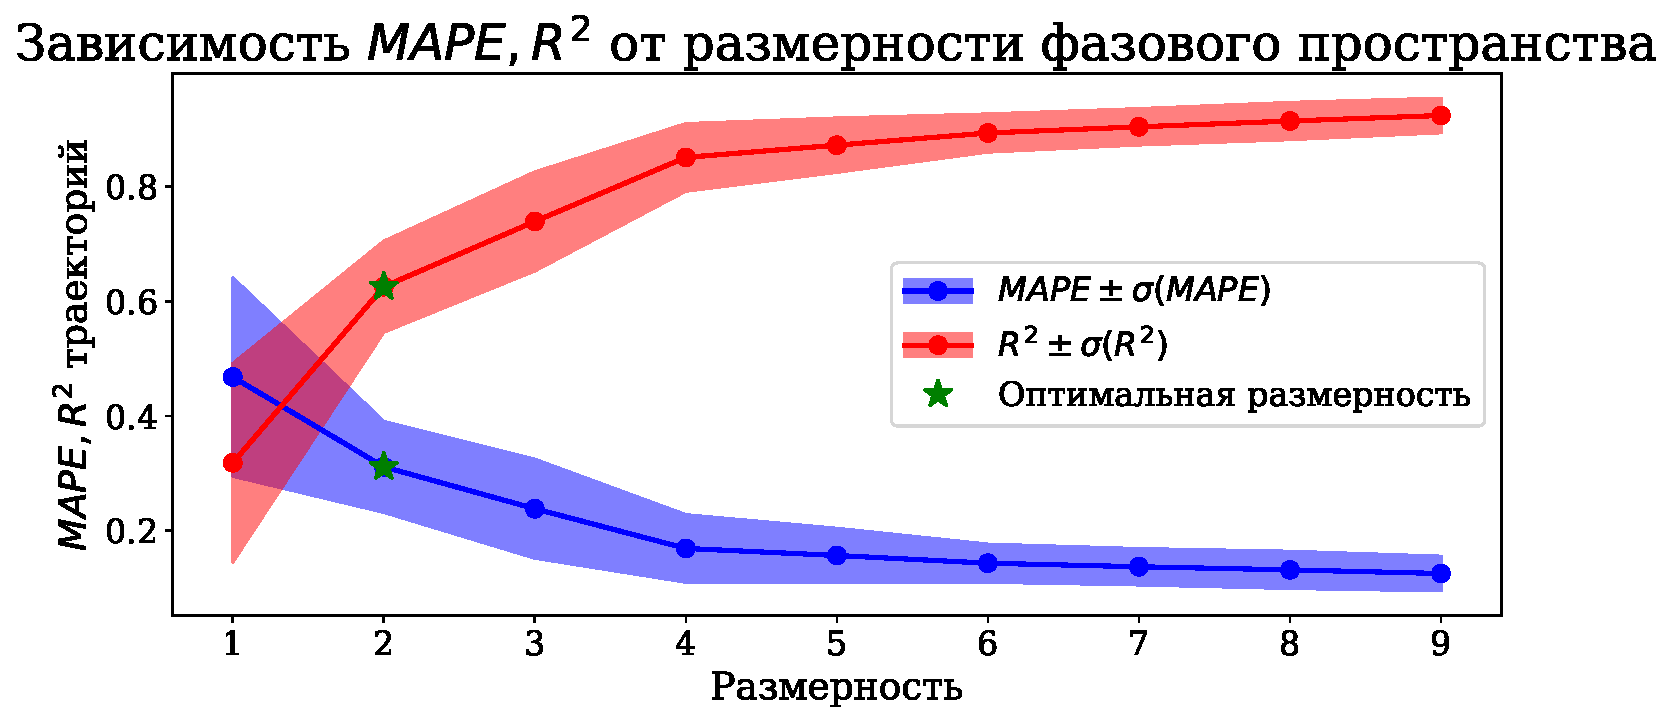
\includegraphics[scale=0.35]{./images/ru_mape_r2_p_bicycle.pdf}\\ 
            \hline
            
            \rotatebox{90}{ \text{Приседания} }
             & 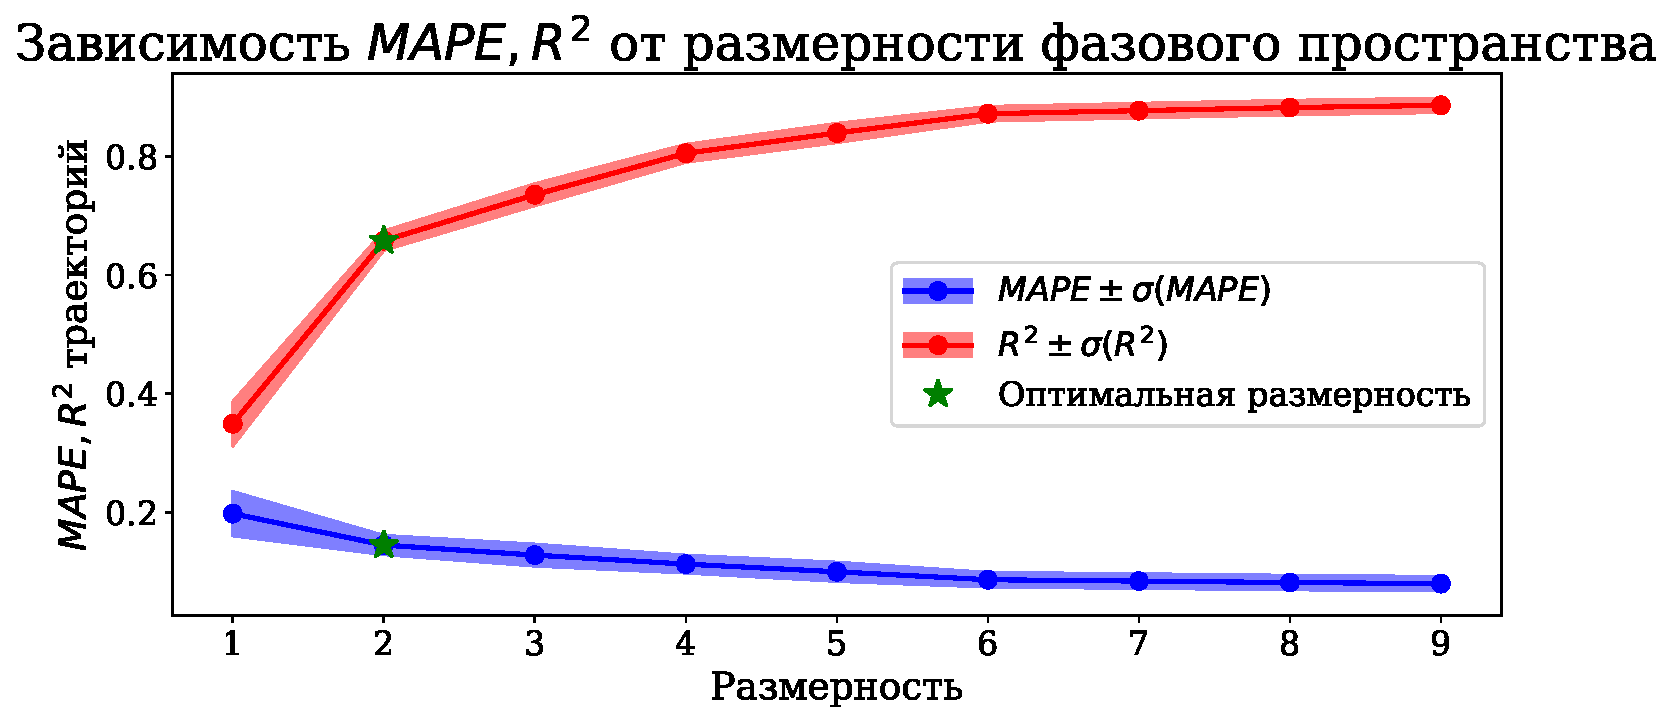
\includegraphics[scale=0.35]{./images/ru_mape_r2_p_squa.pdf}\\ 
            \bottomrule
        \end{tabular}
    \caption{Таблица выбора оптимальной размерности для разных классов движения}
    \label{tbl:table_of_opt_dimension}
\end{table}

Временные ряды, фазовые траектории оптимальных размерностей и результаты работы алгоритма для соответствующих классов движения представлены в таблице \ref{tbl:table_of_figures}. В случае, если оптимальная размерность не превышает 2, то осуществляется переход в трехмерное фазовое подпространство.

\begin{table}
    \centering
        \begin{tabular}{p{0.5cm}p{4cm}p{4cm}p{5cm}}
            \toprule
              & Временной ряд & Фазовая траектория движения & Фаза движения\\
            \midrule
            \rotatebox{90}{ \text{Ходьба} }
            & 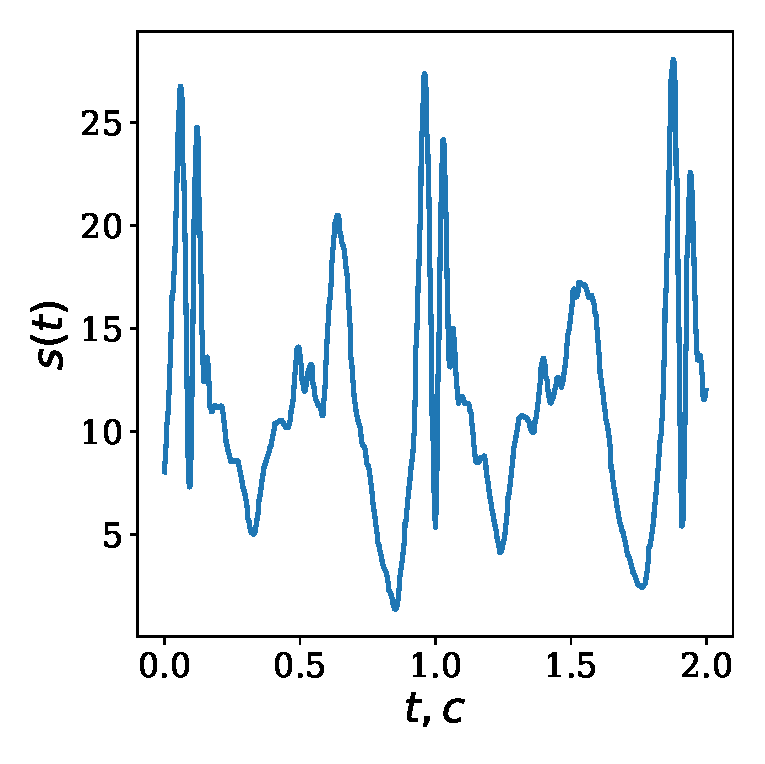
\includegraphics[scale=0.25]{./images/walk_example.eps}
            & 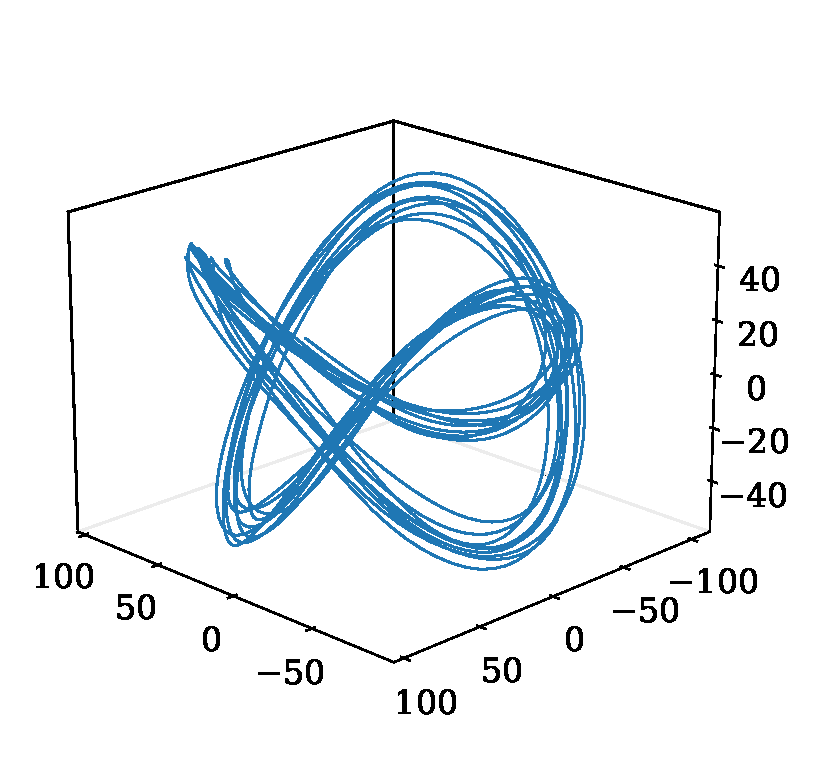
\includegraphics[scale=0.3]{./images/walk_trajectory.eps}
            & 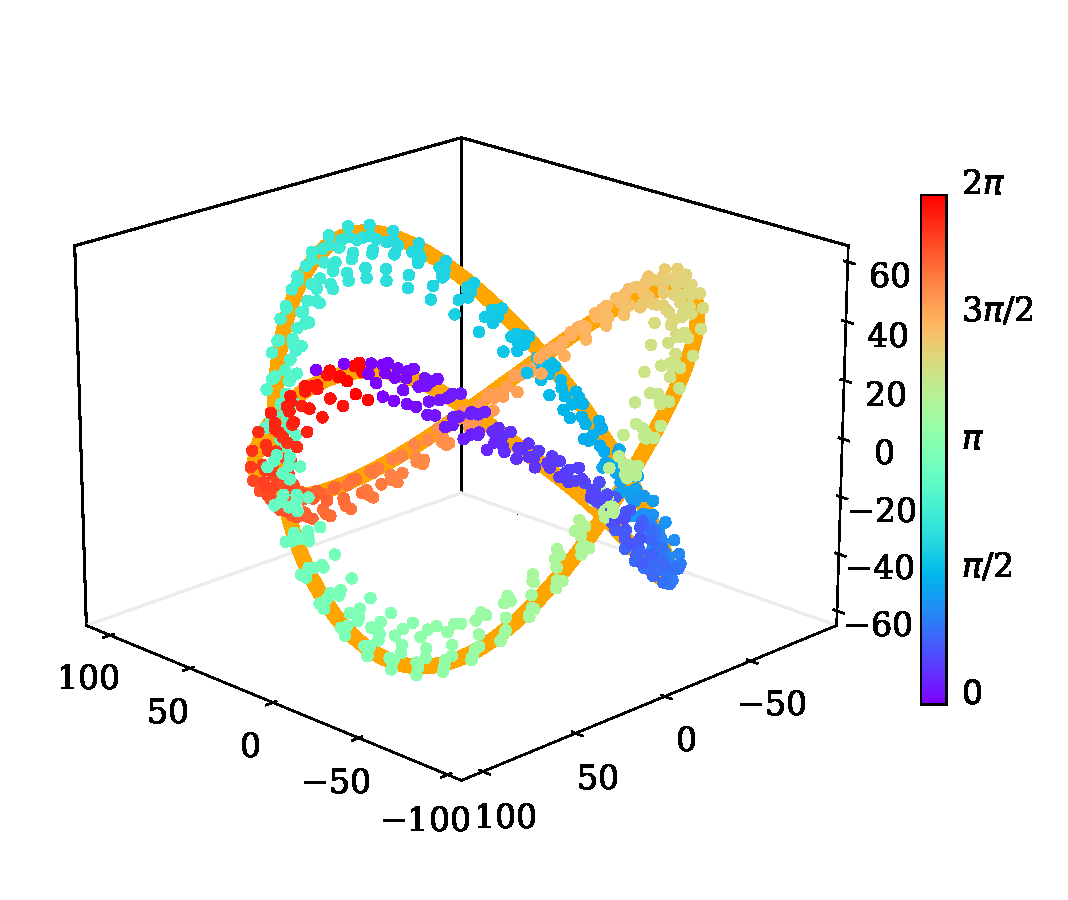
\includegraphics[scale=0.25]{./images/walk_phase.eps} \\ 
            \hline
            
            \rotatebox{90}{ \text{Лестница} }
            & 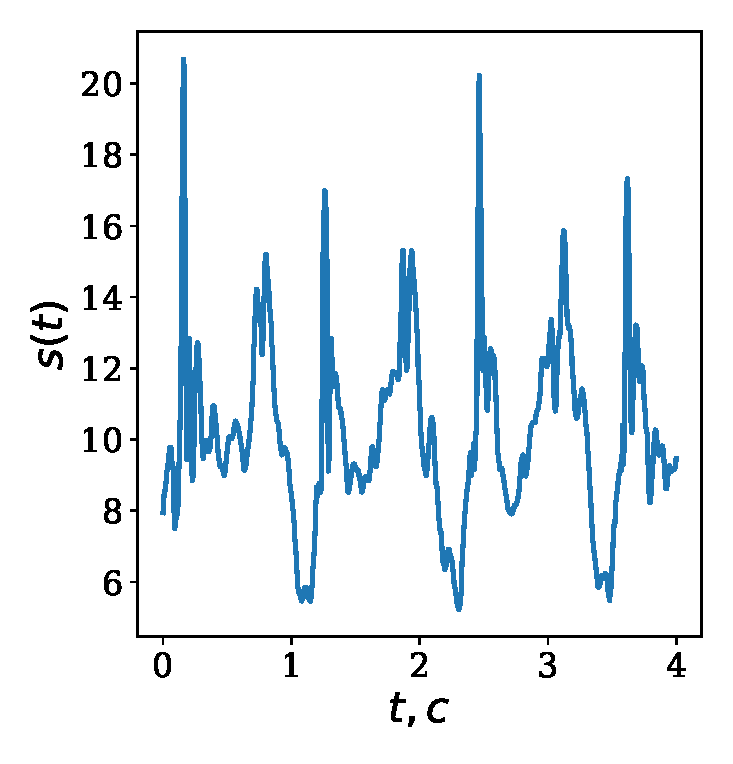
\includegraphics[scale=0.25]{./images/stairs_example.eps}
            & 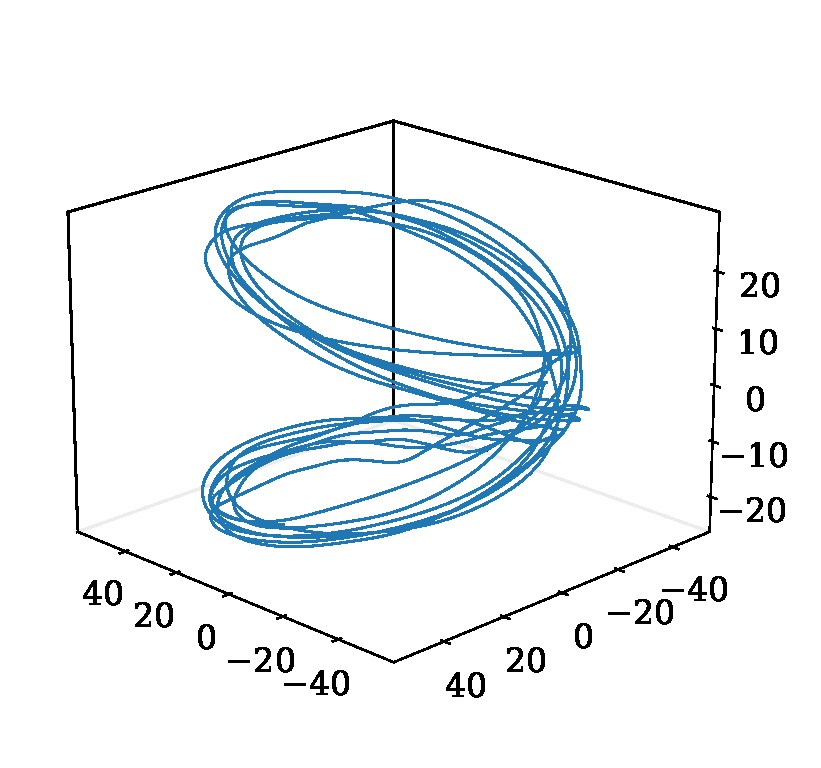
\includegraphics[scale=0.3]{./images/stairs_trajectory.eps}
            & 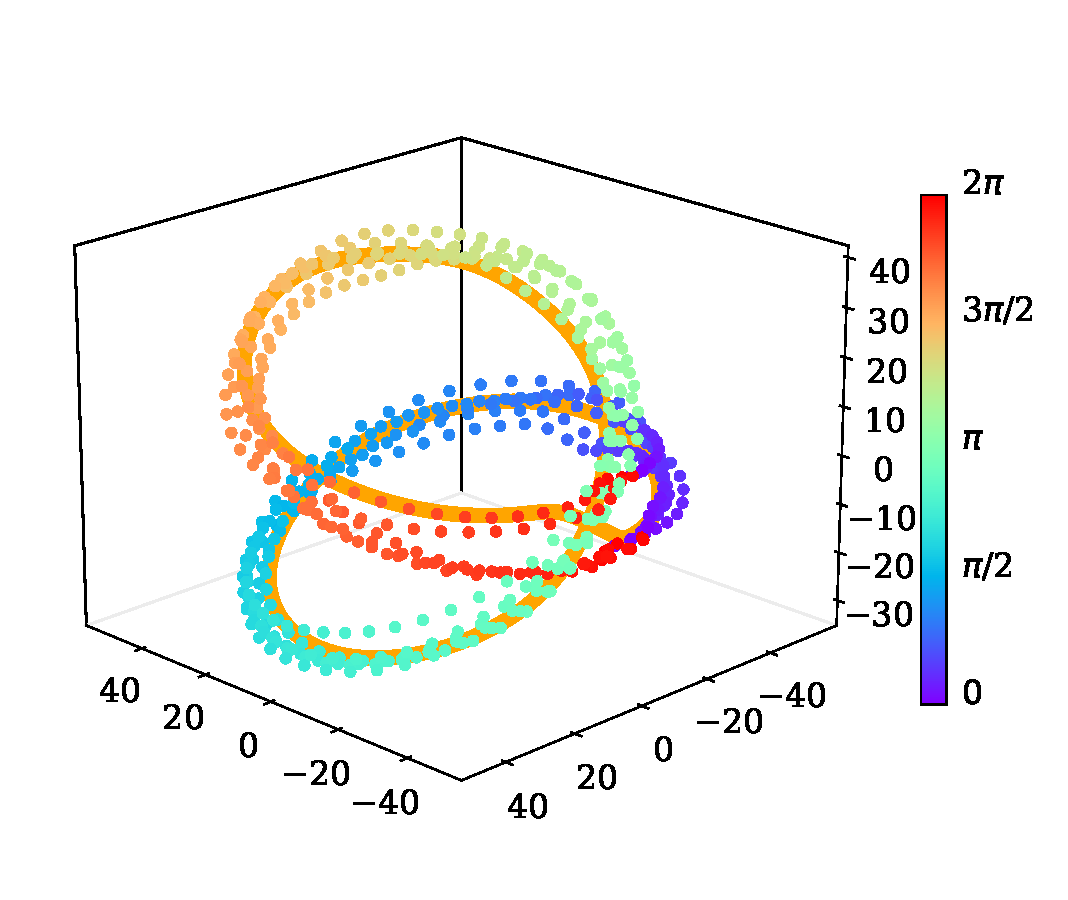
\includegraphics[scale=0.25]{./images/stairs_phase.eps} \\ 
            \hline        
            
            \rotatebox{90}{ \text{Велопрогулка} }
            & 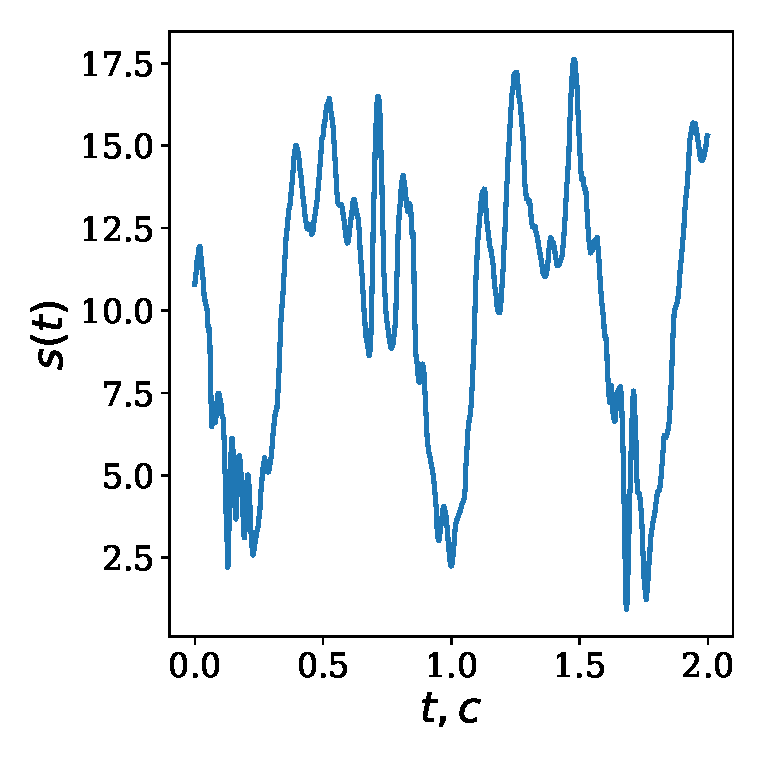
\includegraphics[scale=0.25]{./images/bike_example.eps}
            & 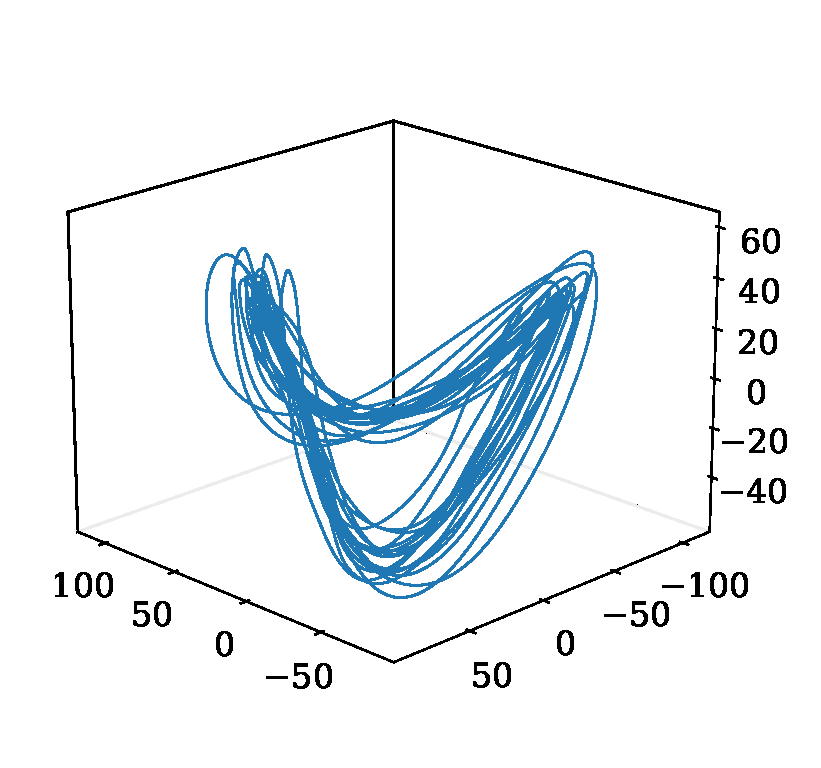
\includegraphics[scale=0.3]{./images/bike_trajectory.eps}
            & 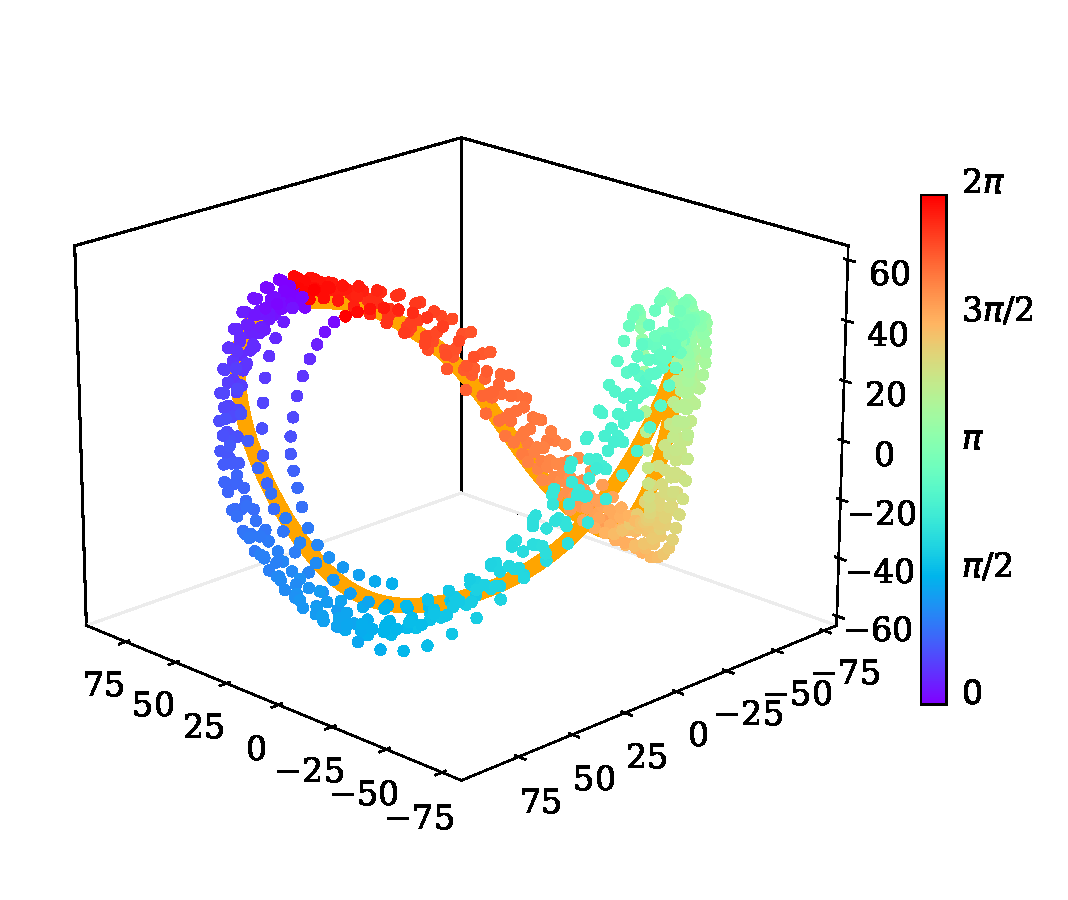
\includegraphics[scale=0.25]{./images/bike_phase.eps} \\ 
            \hline
            
            \rotatebox{90}{ \text{Приседания} }
            & 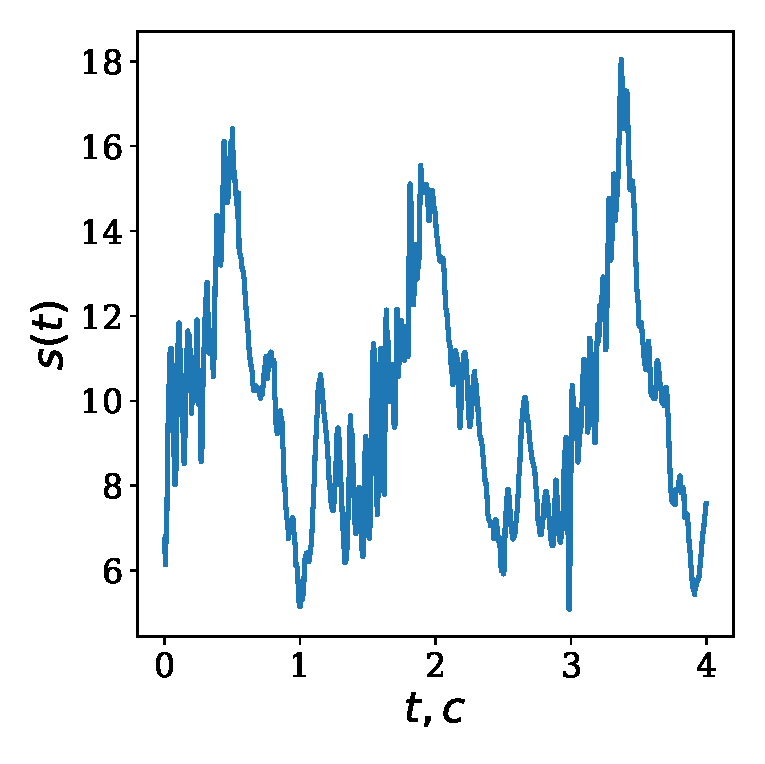
\includegraphics[scale=0.25]{./images/squats_example.eps}
            & 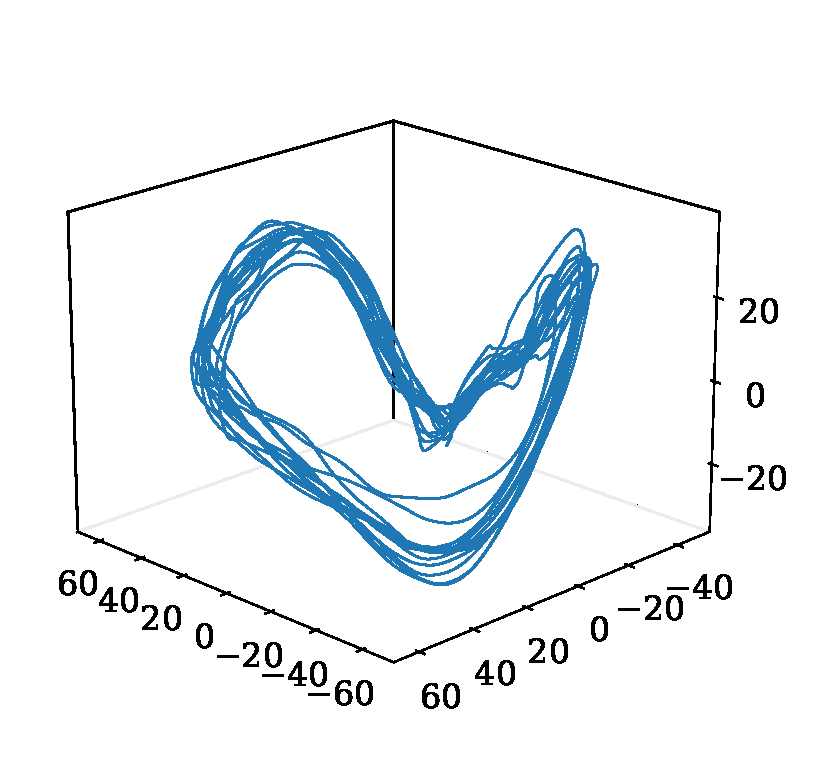
\includegraphics[scale=0.3]{./images/squats_trajectory.eps}
            & 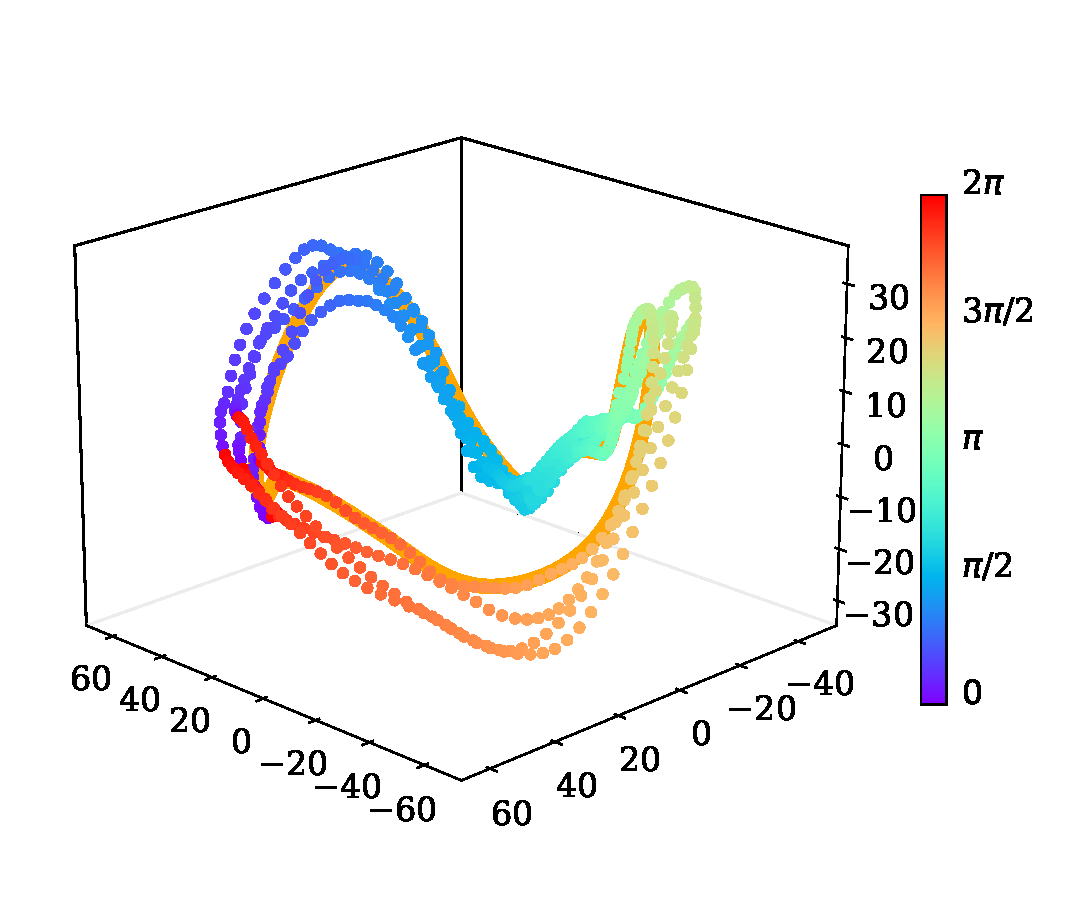
\includegraphics[scale=0.25]{./images/squats_phase.eps} \\ 
            \bottomrule
        \end{tabular}
    \caption{Временные ряды и фазовые траектории в трехмерном представлении для четырех классов движения}
    \label{tbl:table_of_figures}
\end{table}

Сравним таблицу \ref{tbl:table_of_opt_dimension} и таблицу \ref{tbl:table_of_figures}. Так, например, ходьба и движение вверх по лестнице имеют более сложную траекторию в фазовом пространстве, что требует б\'{о}льшей размерности траекторного подпространства. 

%%%%%%%%%%%%%%%%%%%%%%%%%%%%%%%%%%%%%%%%%%%%%%%%%%%%%%%%%%%%%%%%%%%%%%%%%%%%%%%%
\section{Анализ ошибки}
\paragraph{Сравнение на данных акселерометра}
Для анализа эффективности предложенного алгоритма рассматривается сравнение результатов с более простым и интуитивно понятным методом, использующим максимумы автокорреляционной функции. Данный метод заключается в трех последовательных шагах:
    \begin{enumerate}
        \item Применить автокорреляционную функцию к временному ряду
        \item Определить верхние пики автокорреляции
        \item Проставить равномерно фазу от $0$ до $2\pi$ между каждой парой соседних пиков
    \end{enumerate}

\begin{figure}[H]
\begin{minipage}[ht]{0.47\linewidth}
\center{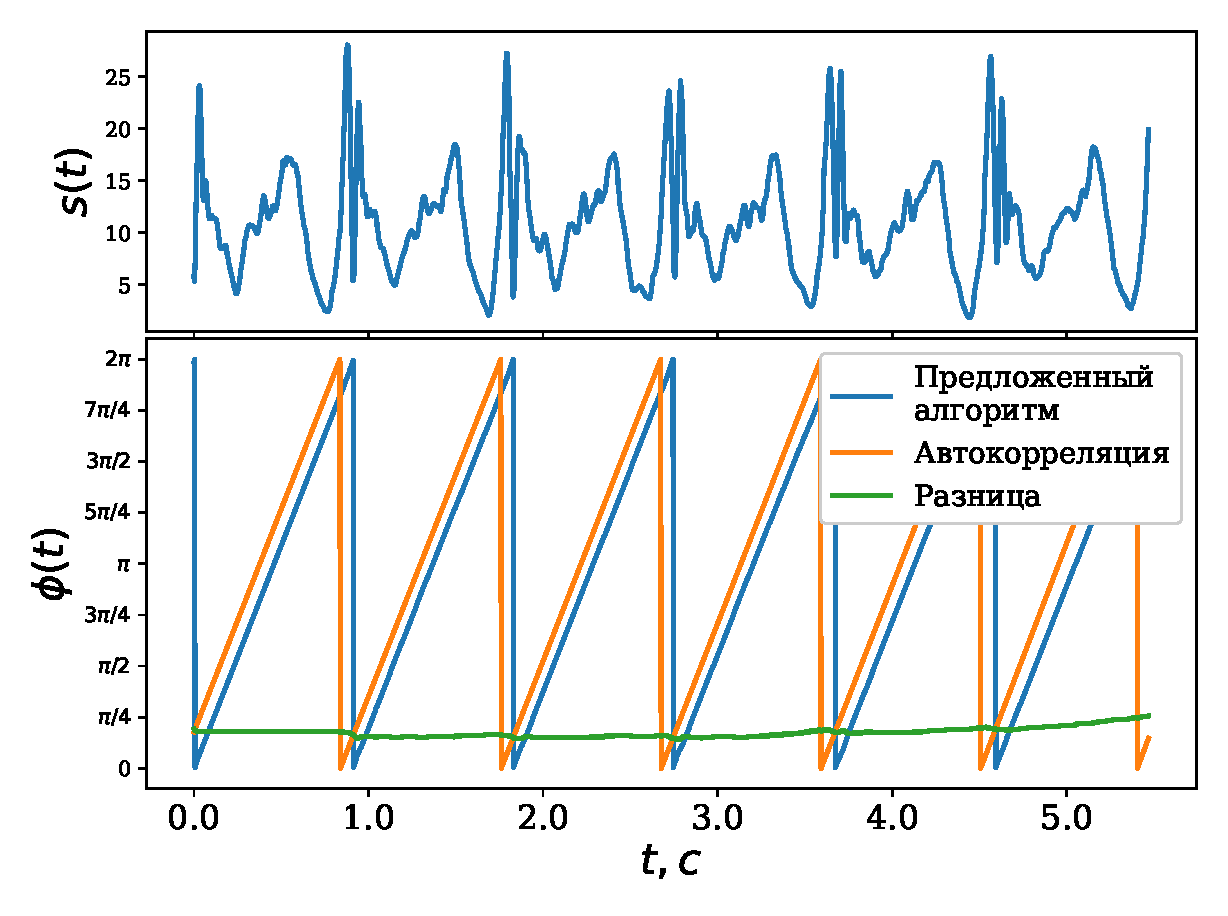
\includegraphics[scale=0.35]{./images/noize_walk.eps}}\\ (а)
\end{minipage}
\hfill
\begin{minipage}[ht]{0.47\linewidth}
\center{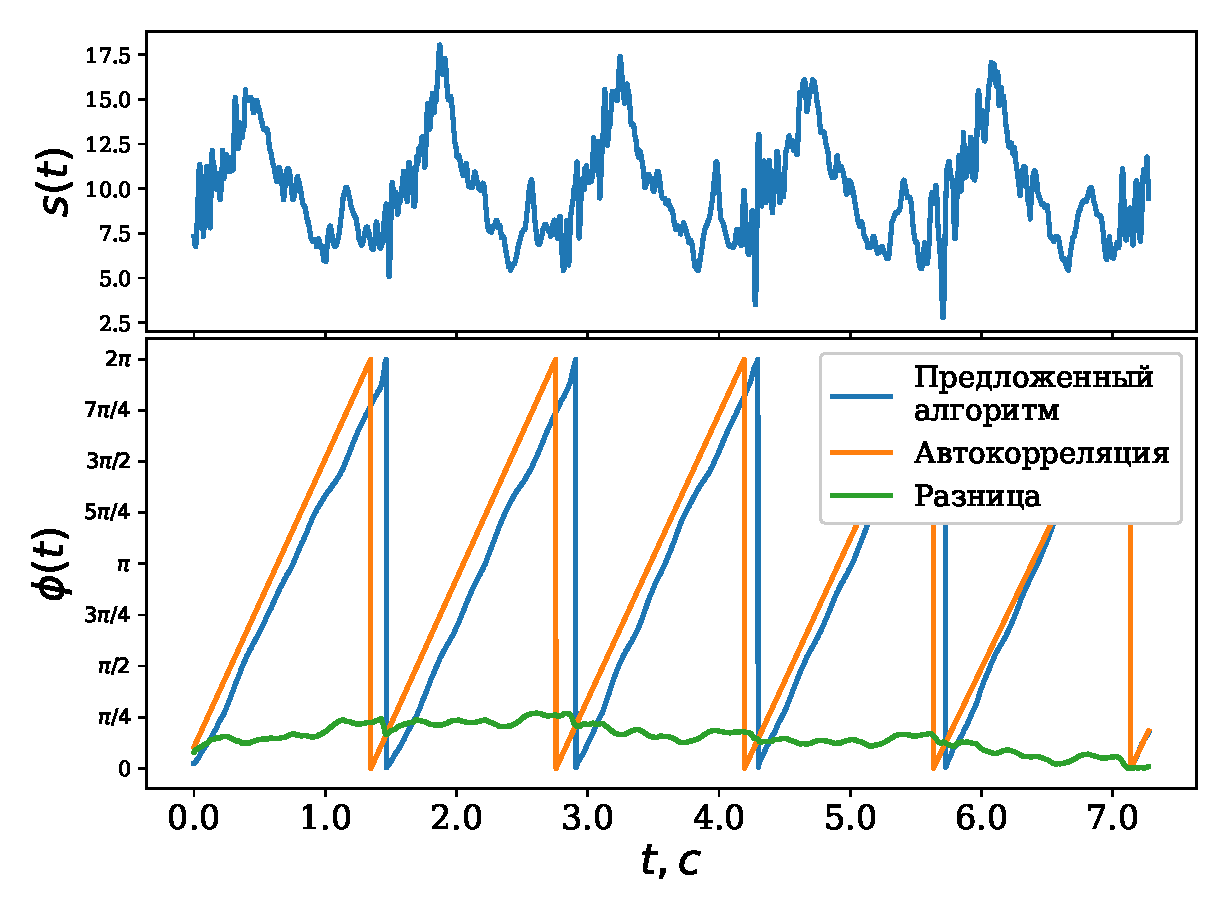
\includegraphics[scale=0.35]{./images/noize_squats.eps}}\\(б)
\end{minipage}
\vfill
\begin{minipage}[ht]{0.47\linewidth}
\center{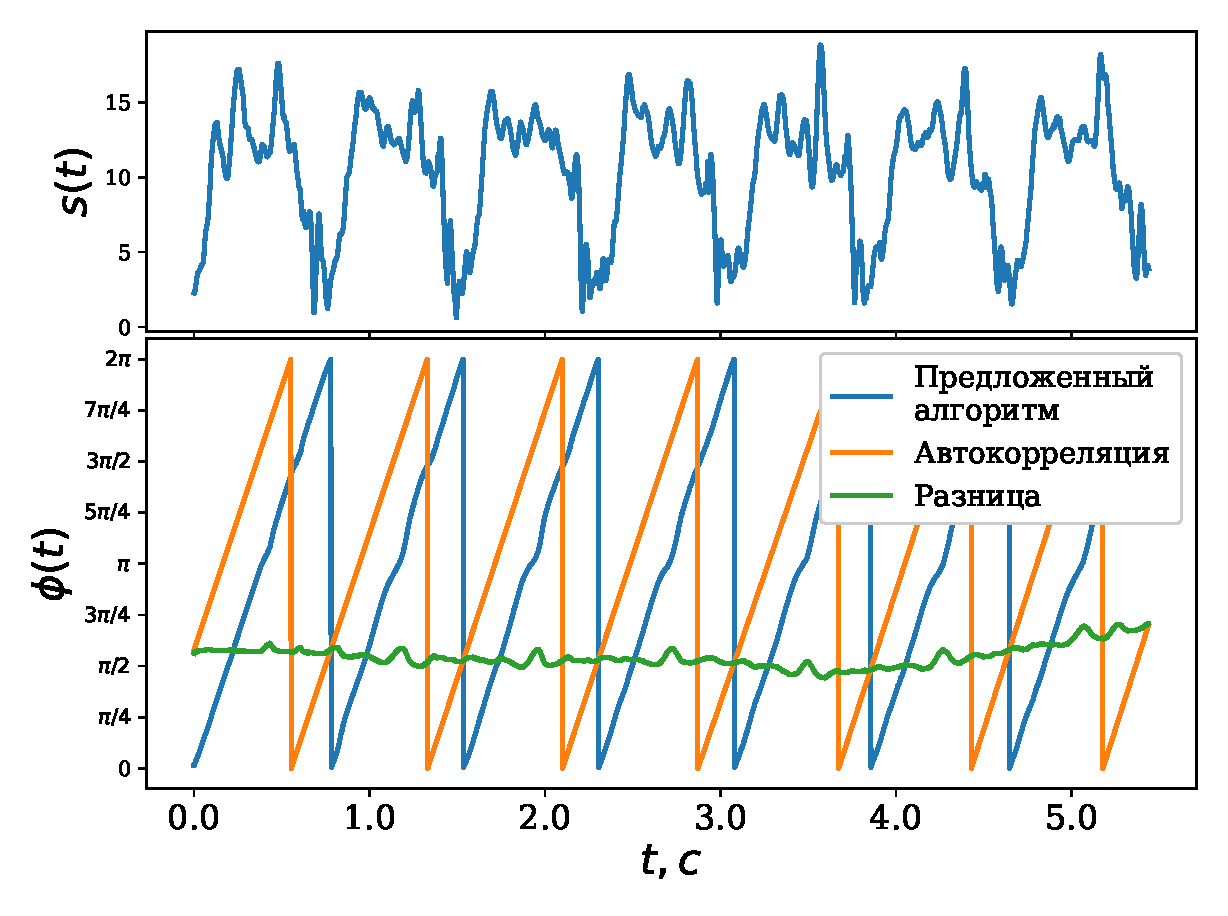
\includegraphics[scale=0.35]{./images/noize_bike.eps}}\\(в)
\end{minipage}
\hfill
\begin{minipage}[ht]{0.47\linewidth}
\center{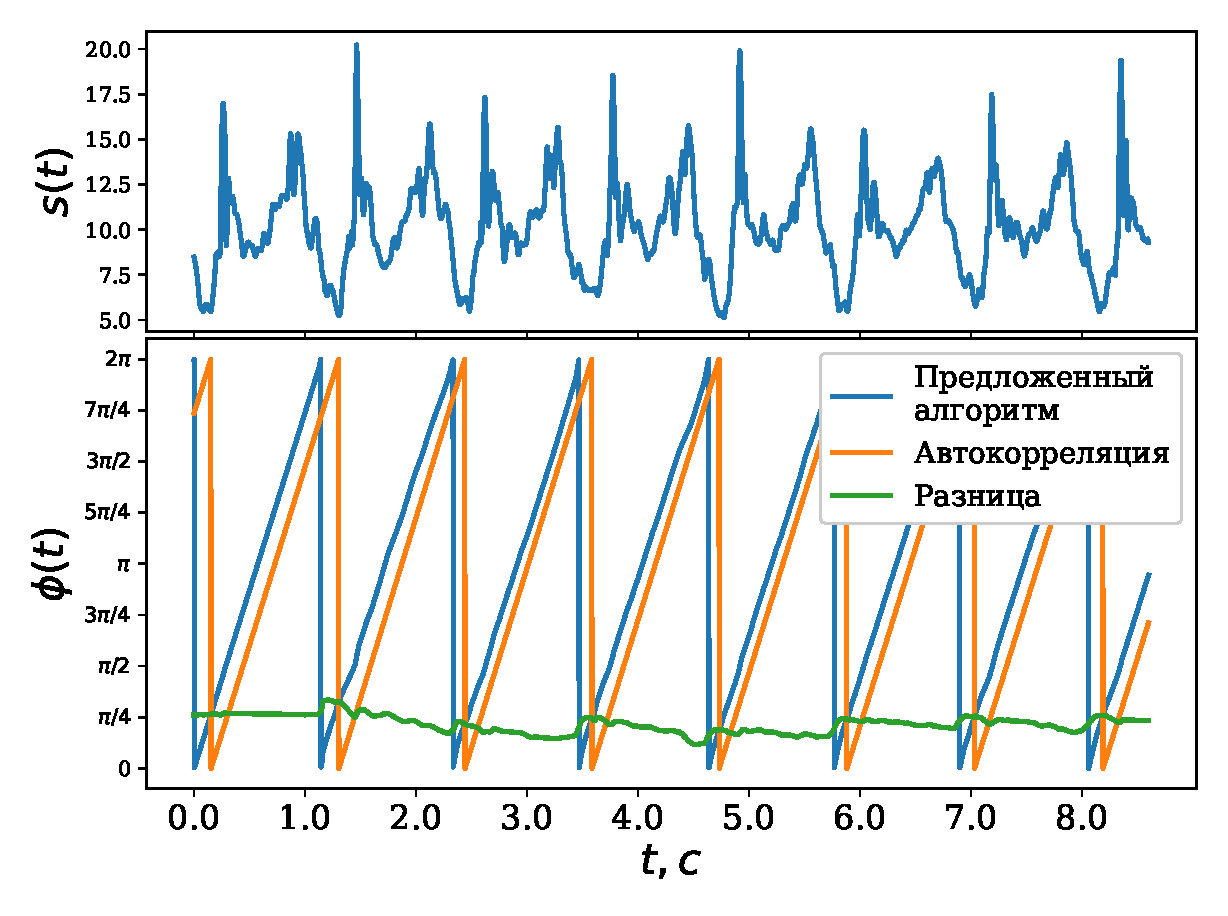
\includegraphics[scale=0.35]{./images/noize_stairs.eps}}\\(г)
\end{minipage}
\caption{Результаты работы в сравнении с пиками автокорреляционной функции: а) ходьба, б) приседания, в) вело-прогулка, г) подъем по лестнице.}
\label{fg:results_comp}
\end{figure}

Анализ результатов сравнения показывает, что предложенный алгоритм имеет ошибку, которая держится на постоянном уровне. Т.е. результат алгоритма имеет ошибку, близкую к нулю, с точностью до сдвига.

\paragraph{Ошибка на сигналах с изменяющимися частотой и амплитудой}
Также были проведены дополнительные эксперименты, демонстрирующие преимущества и недостатки предложенного алгоритма. На рис. \ref{fg:results_comp} ошибка отклоняется от константного уровня в те моменты, когда в исходном временном ряде происходит изменение частоты. Рассмотрим два модельных временных ряда, описывающих изменение амплитуды и частоты:
\abovedisplayskip=0pt
\belowdisplayskip=0pt
\noindent
\begin{gather}
    x_1(t) = \alpha(t)\cdot\sin(\omega t) \label{eq:freq}\\
    x_2(t) = \sin(\beta(t)\cdot \omega t) \label{eq:amplidute},
\end{gather}
где $\alpha(t), \beta(t)$ -- изменяющиеся во времени коэффициенты.

Таким образом, можно сравнивать подходы с истинным значением фазы. Результаты алгоритма на модельных рядах~\eqref{eq:freq},~\eqref{eq:amplidute} продемонстрированы на рис.~\ref{fg:noise_freq} и~\ref{fg:noize_amp} соответственно.
\begin{figure}[ht]
\centering
{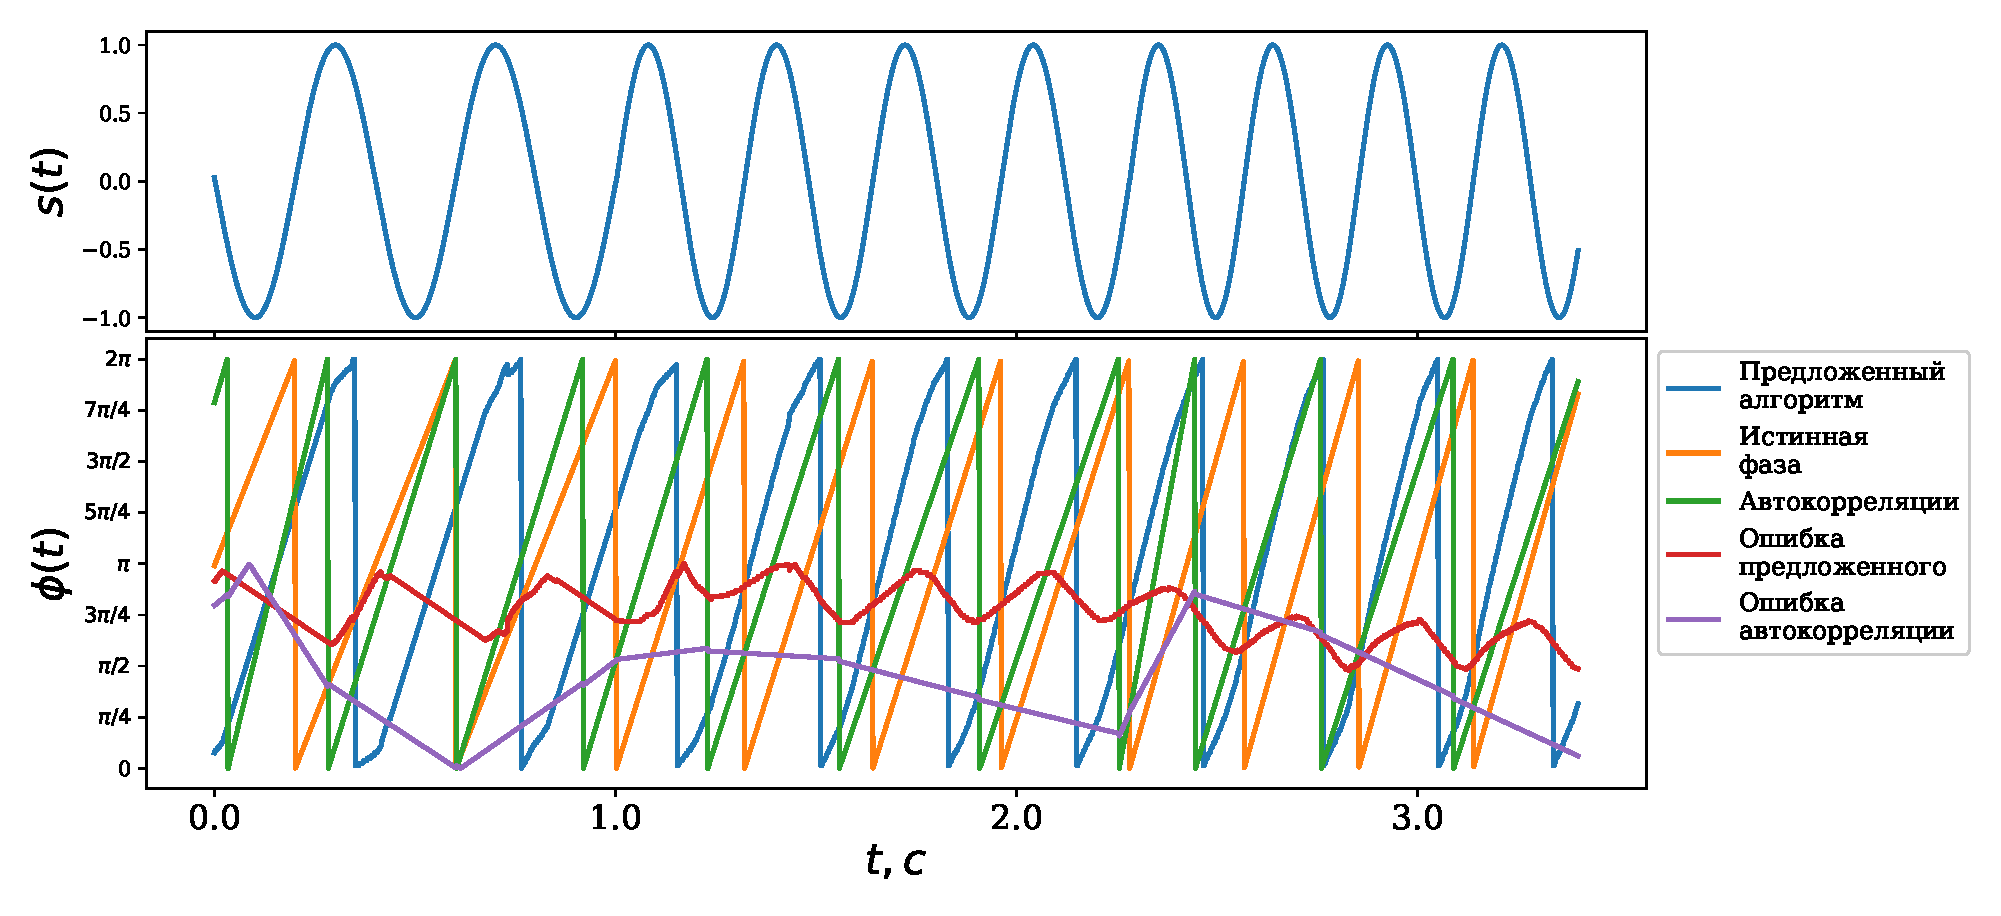
\includegraphics[width=0.9\textwidth]{./images/noize_freq.eps}}

\caption{Временной ряд с изменяющейся частотой}
\label{fg:noise_freq}
\end{figure}
\abovedisplayskip=0pt
\belowdisplayskip=0pt
\noindent
\begin{figure}[ht]
\centering
{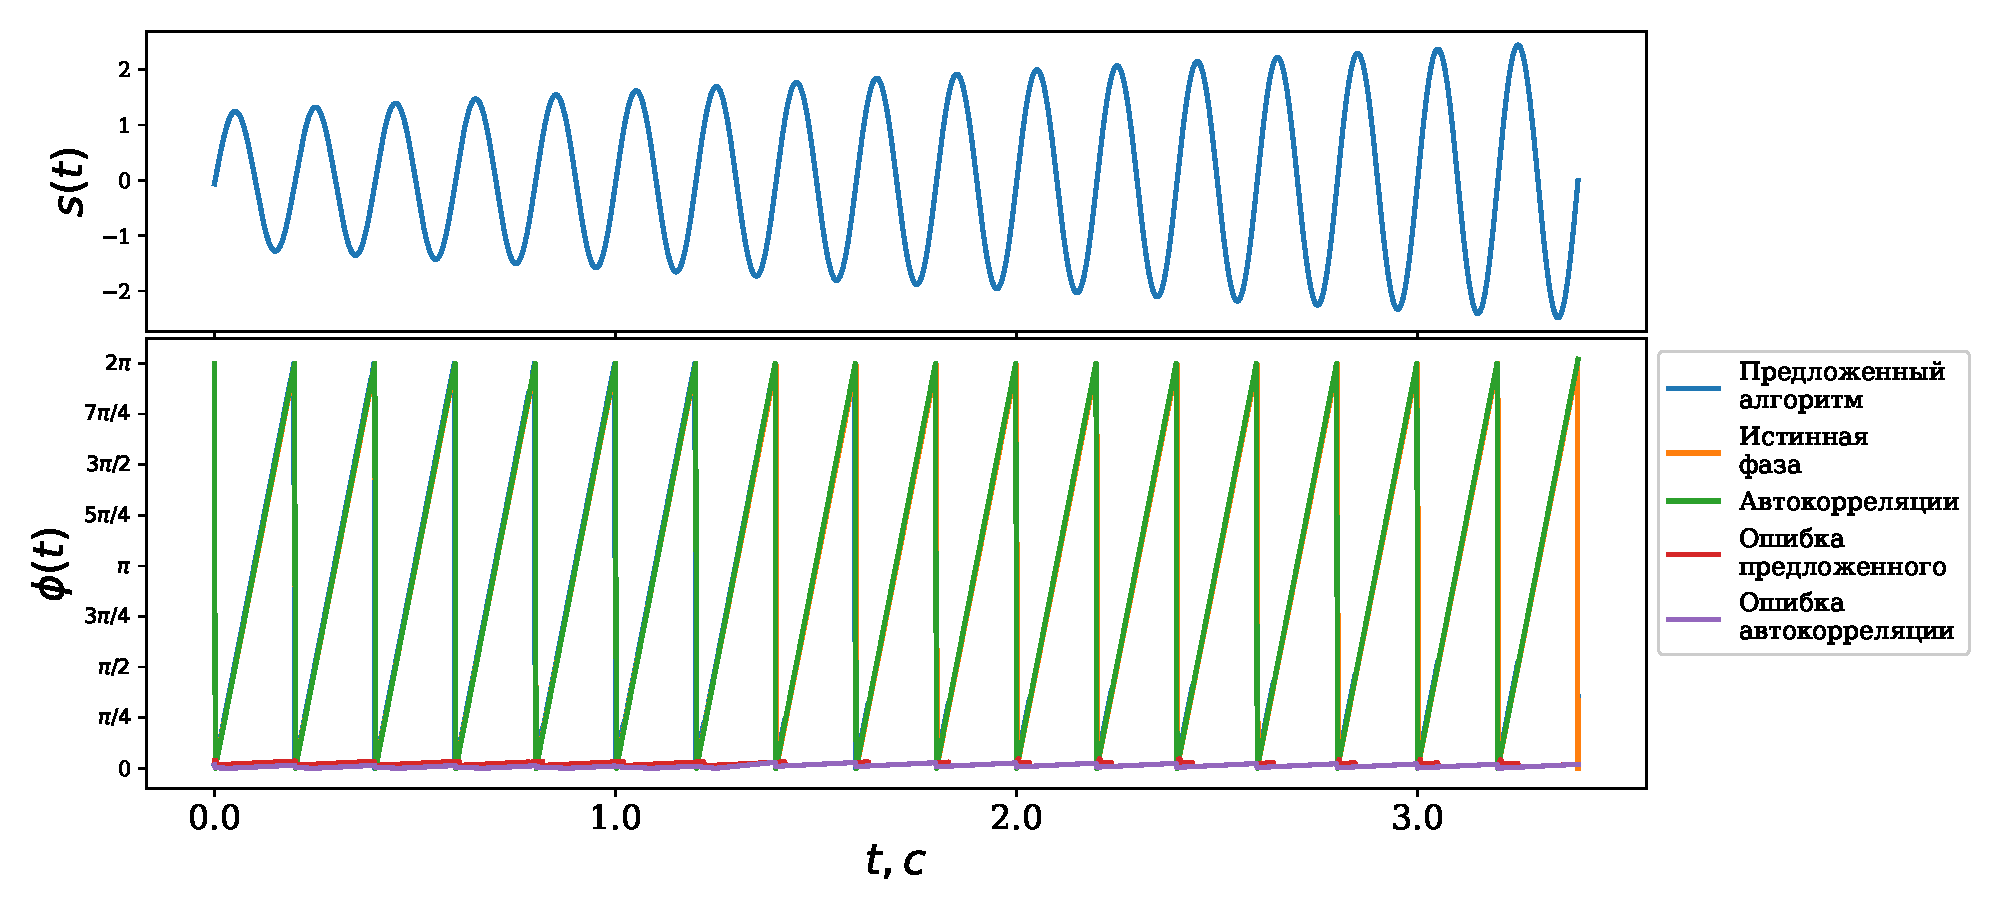
\includegraphics[width=0.9\textwidth]{./images/noize_amp.eps}}

\caption{Временной ряд с изменяющейся амплитудой}
\label{fg:noize_amp}
\end{figure}

На основании приведённых экспериментов можно сделать однозначный вывод об устойчивости предложенного алгоритма к изменению амплитуды. В случае с изменением частоты видно периодическое изменение ошибки результатов модели, свидетельствующее об изменении фазовой траектории исходного временного ряда. При сильных изменениях - это может сделать восстановленную фазу неустойчивой (в смысле ошибки относительно известной истинной фазы).

%%%%%%%%%%%%%%%%%%%%%%%%%%%%%%%%%%%%%%%%%%%%%%%%%%%%%%%%%%%%%%%%%%%%%%%%%%%%%%%%
\section{Заключение}
 
В данной работе была рассмотрена задача восстановления фазы квазипериодического ряда движения человека. Была предложена модель, аппроксимирующая фазовую траекторию. С помощью этой модели был сформулирован критерий оптимальной размерности траекторного подпространства. В пространстве сниженной размерности применяется алгоритм определения фазы, предлагаемый в данной работе.

Был проведен вычислительный эксперимент для четырех типов движения. Определена оптимальная размерность фазового пространства, после чего восстанавливалась фаза временного ряда для каждого типа движения. Качество работы алгоритма сравнивалось с методом максимумов автокорелляционной функции. Дополнительно были проведены исследования устойчивости алгоритма к изменениям частоты и амплитуды исходного ряда на модельных примерах. 
%%%%%%%%%%%%%%%%%%%%%%%%%%%%%%%%%%%%%%%%%%%%%%%%%%%%%%%%%%%%%%%%%%%%%%%%%%%%%%%%
%%%% если имеется doi цитируемого источника, необходимо его указать, см. пример в \bibitem{article}
%%%% DOI публикации, зарегистрированной в системе Crossref, можно получить по адресу http://www.crossref.org/guestquery/
%%%%%%%%%%%%%%%%%%%%%%%%%%%%%%%%%%%%%%%%%%%%%%%%%%%%%%%%%%%%%%%%%%%%%%%%%%%%%%%%
\bibliographystyle{unsrt}
\bibliography{biblio}


\end{document} 